%%%%%%%%%%%%%%%%%%%%%%%%%%%%%%%%%%%%%%%%%
% Report Template
% LaTeX Template
% Version 1.1 (2023-04-19)
%
% This template was adapted by:
% Jonathan Decker (jonathan.decker@uni-goettingen.de)
% Adapted from the informatics master and bachelor thesis template
% offered by the University Göttingen
% https://www.uni-goettingen.de/de/626775.html
%
%%%%%%%%%%%%%%%%%%%%%%%%%%%%%%%%%%%%%%%%%
\documentclass[12pt, a4paper, hidelinks]{article}

\usepackage{graphicx}
\usepackage{hyperref}
\usepackage{xcolor}
\usepackage[english]{babel}
\usepackage[nottoc]{tocbibind}
\usepackage[utf8]{inputenc}
\usepackage[T1]{fontenc}
\usepackage[backend=biber,style=numeric,sorting=none]{biblatex}
\addbibresource{ref.bib} % The filename of the bibliography
\usepackage[left=2.5cm,right=2.5cm,top=2.5cm,bottom=2.5cm]{geometry}
\usepackage{acronym}
\usepackage{fancyhdr}
\pagestyle{fancy}
\usepackage{lipsum}
\usepackage{array, tabularx, booktabs} % For better tables
\usepackage{longtable}
\usepackage{minted}
\usemintedstyle{tango}
\setminted{linenos, autogobble, bgcolor=gray!5}
\usepackage{amssymb}
\usepackage{amsthm}
\usepackage{amsmath}
\usepackage{amsfonts}
\usepackage{cleveref}
\usepackage{titlesec}
\setlength{\marginparwidth}{2cm}
\usepackage{todonotes}
\usepackage[autostyle=true]{csquotes}
\usepackage{tikz}
\usetikzlibrary{graphs.standard}
\usepackage{tikz-qtree}
\usepackage{caption} % subfigure
\usepackage{subcaption} % subfigure

\iffalse

\definecolor{codegreen}{rgb}{0,0.6,0}
\definecolor{codegray}{rgb}{0.5,0.5,0.5}
\definecolor{backcolour}{gray}{0.95}
\definecolor{codeorange}{rgb}{0.8,0.5,0.2}

\definecolor{bluekeywords}{rgb}{0.13, 0.13, 1}
\definecolor{greencomments}{rgb}{0, 0.5, 0}
\definecolor{redstrings}{rgb}{0.9, 0, 0}
\definecolor{graynumbers}{rgb}{0.5, 0.5, 0.5}

\usepackage{listings}
\lstset{
    autogobble,
    columns=fullflexible,
    showspaces=false,
    showtabs=false,
    breaklines=true,
    showstringspaces=false,
    breakatwhitespace=true,
    escapeinside={(*@}{@*)},
    commentstyle=\color{greencomments},
    keywordstyle=\color{bluekeywords},
    stringstyle=\color{redstrings},
    numberstyle=\color{graynumbers},
    basicstyle=\ttfamily\footnotesize,
    frame=l,
    framesep=12pt,
    xleftmargin=12pt,
    tabsize=4,
    captionpos=b
}

\fi

\titleformat{\section}[hang]{\huge\bfseries}{\thesection\hspace{20pt}}{0pt}{\huge\bfseries}
\graphicspath{{figures/}{./}{assets/}}

\newcommand{\ccheckmark}{\mbox{\ooalign{$\checkmark$\cr\hidewidth$\square$\hidewidth\cr}}}
\newcommand{\ccheckbox}{\mbox{$\square$}}

% --- document configuration ---

\newcommand{\thesistitle}{Rusty Parallel Traveling Salesman Problem Solver}
\newcommand{\supervisor}{Dr. Artur Wachtel}
\newcommand{\authorname}{Lars Quentin, Johann Carl Meyer}
\newcommand{\university}{Georg-August-Universität Göttingen}
\newcommand{\department}{Institute of Computer Science}
\newcommand{\thesistype}{Seminar Report}
\newcommand{\matrikelnumber}{21774184, 21969570}
\newcommand{\keywords}{} % Set keywords that describe your report

\hypersetup{pdftitle=\thesistitle} % Set the PDF's title to your title
\hypersetup{pdfauthor=\authorname} % Set the PDF's author to your name
\hypersetup{pdfkeywords=\keywords} % Set the PDF's keywords to your keywords

% ~~~~~ math definitions ~~~~~~~~~~~~~~~~~~~~~~~~~~~~~

\newcommand{\RR}{\mathbb{R}}
\newcommand{\CC}{\mathbb{C}}
\newcommand{\NN}{\mathbb{N}}
\newcommand{\ZZ}{\mathbb{Z}}

\theoremstyle{plain}
\newtheorem{theorem}{Theorem}[section]
\newtheorem{lemma}[theorem]{Lemma}

\newtheorem{hypothesis}[theorem]{Hypothesis}


%\theoremstyle{definition} % bessere Umrandung von Definitionen? soll sich vom Fließtext abheben
\newtheorem{definition}[theorem]{Definition}
\newtheorem{example}[theorem]{Example}

\theoremstyle{remark}
\newtheorem*{remark}{Remark}

% make multiple-letter function names pretty in math environments
%\DeclareMathOperator{\myfunc}{myfunc}

% ~~~~~~~~~~~~~~~~~~~~~~~~~~~~~~~~~~~~~~~~~~~~~~~~~~~~

\begin{document}

\fancyhead{}
\fancyhead[R]{\footnotesize \thesistitle}
\fancyfoot{}
\fancyfoot[R]{\thepage}
\fancyfoot[L]{Section \thesection}
\fancyfoot[C]{\authorname}
\renewcommand{\headrulewidth}{0.4pt}
\renewcommand{\footrulewidth}{0.4pt}

\pagestyle{plain}
\input{content/titlepage}

% --- abstract ---

%\thispagestyle{empty}
\newpage
\pagenumbering{roman}
\setcounter{page}{1}

\section*{Abstract}
The \ac{TSP} is one of the most studied problems in computer science and one of the most intuitive and well-known NP-complete problems. This report presents walky, a new Rust-based \ac{TSP} solver. Walky supports exact solving using several highly optimized algorithms with support for sequential, multithreaded as well as distributed, MPI execution. Additionally, it supports two different approximation algorithms: The simple, easy-to-implement Nearest Neighbour approximation and the more sophisticated Christofides algorithm. Walky is fully production-ready, fully tested, and supports the most-used TSPLIB-XML format.

The Benchmarks show that, for exact solving, walky successfully uses pruning to immensely improve performance and increase the viability of exact solving. The nearest neighbour algorithm scales well with parallelism due to its minimal inter-worker communication requirements. The 1-tree lower bound also greatly benefits from parallelism. Christofides algorithm in its randomized implementation is a very quick
approximation to the TSP, it can be made more reliable by
utilizing parallelism. For the MST computation, the graphs tested in this setting were
too small to benefit from parallelism, though the benchmarks indicated that for larger
graphs a parallel implementation of Prim’s algorithm would outperform its sequential
counterpart.

Overall, walky shows that Rust is a valid choice for developing highly distributed \ac{HPC} applications.


%\thispagestyle{empty}
% --- table of contents ---
% Comment out the lists you are not using
\newpage

\vfill

\subsection*{Statement on the usage of ChatGPT and similar tools\\ in the context of examinations}
\noindent In this work I have used ChatGPT or a similar AI-system as follows:
\begin{itemize}
	\item[\ccheckbox]  Not at all
	\item[\ccheckmark] In brainstorming
	\item[\ccheckbox] In the creation of the outline
	\item[\ccheckbox] To create individual passages, altogether to the extent of 0\% of the whole text
	\item[\ccheckbox] For proofreading
	\item[\ccheckbox] Other, namely: -
\end{itemize}
I assure that I have stated all uses in full.\\
Missing or incorrect information will be considered as an attempt to cheat.

\vfill

\newpage

\clearpage
\phantomsection\pdfbookmark{\contentsname}{toc}
\tableofcontents

\newpage
\clearpage\phantomsection
\listoftables
%\newpage
%\clearpage
\phantomsection
\listoffigures
%\newpage
%\clearpage
\phantomsection

% if you have abbreviations
\newpage

\section*{List of Abbreviations} \addcontentsline{toc}{section}{List of Abbreviations}
\begin{acronym}[Bash] % Add acronyms such that they are shown in full only on first occurrence
    \acro{API}{Application Programming Interface}
    \acro{CLI}{Command Line Interface}
    \acro{DSL}{Domain Specific Language}
    \acro{HPC}{High-Performance Computing}
    \acro{JSON}{JavaScript Object Notation}
    \acro{MPI}{Message Passing Interface}
    \acro{NDJSON}{Newline Delimited JSON}
    \acro{NIC}{Network Interface Card}
    \acro{SLURM}{Simple Linux Utility for Resource Management}
\end{acronym}


\thispagestyle{plain}
\newpage

% --- content ---

\pagenumbering{arabic}
\setcounter{page}{1}
\pagestyle{fancy}

%\section{Introduction}
\subsection{Motivation}
In the space of \ac{HPC}, a significant trend from more compute-intensive tasks to more data-intensive tasks is taking place. This change necessitates better data-management tooling such as data lakes or data warehouses. Given that \ac{HPC} computes on raw data, data lakes are a more natural fit. Efficient metadata management requires a great metadata store as well as support for full-text searches.

In this report, the viability of Elasticsearch\footnote{\url{https://www.elastic.co/elasticsearch}} for \ac{HPC} load is being evaluated. Elasticsearch benefits from many years of tooling development, making it a more pragmatic choice than building an own application around full-text search engines like Apache Lucene\footnote{\url{https://lucene.apache.org/}} or Tantivy\footnote{\url{https://github.com/quickwit-oss/tantivy}}.

While elastic provides rally\footnote{\url{https://github.com/elastic/rally}}, an in-house benchmark suite used for performance regression testing \cite{es_benchmarking}, after rigorous internal testing it was found out that thespian\footnote{\url{https://thespianpy.com/doc/}}, its internal actor framework, did not scale up to more than 60 nodes, which was not sufficient for previous large-scale stress testing. Thus, for this report a new benchmarking framework was designed, using reliable \ac{HPC} native technologies such as \ac{MPI}.

In addition, the data lake related use cases at the GWDG include spawning Elasticsearch instances on-demand. For this dynamic deployment, a containerized Elasticsearch cluster based on the underlying \ac{SLURM}\footnote{\url{https://slurm.schedmd.com/documentation.html}} and \ac{MPI} are needed. It should auto-configure itself, in order to be IP-agnostic.
\subsection{Goals and Contributions}
The goals of this report are twofold: First, providing and implementing a stateful architecture to dynamically spawn and respawn an Elasticsearch cluster without any previous manual configuration. Second, design a highly-scalable, \ac{HPC}-native, distributed Elasticsearch benchmarking framework for both ingestion and querying performance. 

To achieve these goals, the following contributions were made:

\begin{itemize}
\item Design and implementation of a zero-configuration workflow to spawn a rootless, containerized Elasticsearch cluster of arbitrary size within a SLURM-allocated \ac{MPI} environment.
\item Design and implementation of a highly scalable, distributed benchmarker for ingestion performance
\item Design and implementation of a highly scalable, distributed benchmarker for query performance with custom benchmark scenarios using a \ac{JSON}-based \ac{DSL}.
\item Benchmark a dynamically spawned Elasticsearch cluster on \ac{HPC} using a canonical dataset common in existing literature.
\end{itemize}
\subsection{Structure}
This report is structured as follows: In section 2, Elasticsearch, the full-text search engine and NoSQL database used, is introduced. After that, section 3 covers the related work starting with classical load generation before focussing on the literature around Elasticsearch benchmarking. In section 4, the methodology and design of all components are covered. First, it covers the design and internal workflow of the aforementioned cluster spawning mechanism. Then, it covers both the ingestion and query benchmarkers. Lastly, it focuses on the benchmark design by showing the steps required to perform the benchmarks and the reasoning behind the corpus and query design used in this specific benchmark. Lastly, in section 5 the results of the benchmark are shown, before describing the open problems and challenges in Chapter 6. Concluding in Chapter 7, the results are summarized and possible future work is shown.

\section{Background}
\subsection{Elasticsearch}
Elasticsearch is a distributed search engine initially developed in 2010. Since it stores its data in a document model, it can also be seen as a NoSQL database. The full-text search internally relies on the Apache Lucene library. It is mainly used for its full-text fuzzy search capabilities and its \ac{JSON}-based REST interface. It is used by many large websites such as Wikipedia\footnote{Wikipedia also used Lucene beforehand.}, Netflix, Stackoverflow, and LinkedIn.

In Elasticsearch, a collection of \emph{documents} are stored in an \emph{index}. Documents are equivalent to, and can be sent in the form of, \ac{JSON} objects. They can be nested. Each index has a \emph{schema}, which is a type mapping for each of the key-value pairs contained in the index\footnote{Akin to a SQL database definition.}. This mapping can either be statically preconfigured or dynamically guessed at ingestion time. The index data can be \emph{queried} using Elasticsearchs own \ac{DSL}, again relying on \ac{JSON} and REST as the foundational technology.

In 2021, due to a license change from Apache 2.0 to a more permissive license, OpenSearch was created as an Elasticsearch fork, which is maintained by several companies such as AWS.

\section{Related Work}
While the topic of Elasticsearch benchmarking is more sparsely covered, a lot of previous work around general HTTP API benchmarking exists. The most used load generator is Apache JMeter \cite{jmeter}, a sophisticated graphical load tester that supports many protocols such as HTTP(S), SOAP, or LDAP. Only relying on the \ac{CLI} interface, wrk \cite{wrk} provides a simpler popular alternative. For a more scriptable alternative, the Javascript-based Grafana k6 \cite{k6} gained a lot of popularity over recent years.\\

For benchmarking Elasticsearch, the main tool is the aforementioned rally \cite{rally}, a microbenchmarking framework developed by Elastic. While it can be run on a single node, it also supports distributed benchmarking through the Thespian actor system.

Different benchmarking scenarios are defined as so-called \emph{tracks}. Every track contains one or more \emph{corpora}, containing \ac{NDJSON} objects as documents. All tracks are available on GitHub \cite{rallytracks}. Each track contains many \emph{operations} such as ingestion or specific queries, which are then structured into a \emph{challenge's} \emph{schedule} in a fork-join model. This means that Rally can be extended without editing the source code.

The rally framework is actively used in literature for benchmarking Elasticsearch clusters \cite{rallyusecase1} \cite{rallyusecase2} \cite{rallyusecase3}. As mentioned in the introduction, it was not a viable choice for this paper due to the underlying actor framework not scaling into more than 128 nodes in previous experiments.

Furthermore, most of the benchmark comparisons between NoSQL databases such as tsbs \cite{tsbs} are done by database vendors themselves, resulting in conflicting financial interests.

\section{Methodology and Design}
The Methodology and Design section is split into four parts: First, the autoconfigured Elasticsearch cluster spawner is presented. After that, the next two subsections cover the distributed ingestion and query benchmarker respectively, including underlying reasoning as well as some technical details. Lastly, the overall benchmark design used for this report is discussed, focusing mainly on the high-level benchmark workflow as well as the corpus and query design.

\subsection{Dynamic Cluster Creation Based on MPI Communicator}
This section presents an automated approach to configuring and spawning a multi-node Elasticsearch cluster based solely on the \ac{MPI} environment set up by SLURM. It dynamically fetches the different hosts, i.e. it is not required to know the hostnames or IPs beforehand, making it easily embeddable in any kind of job system. The cluster is very portable since it is using Singularity \cite{singularity} containers as an Elasticsearch host. Any cluster size larger or equal to two nodes is supported. The code can be found on GitHub \cite{myspawner}.

Furthermore, it supports \emph{statefulness}, which means that the same cluster can be re-spawned on other nodes\footnote{With the same cluster size.} without requiring a re-ingest, i.e. keeping the complete cluster state and configuration. Due to the aforementioned containerization, this also works while changing both the hardware and IP addresses. The only limitation is that it only supports one Elasticsearch node per host OS. This is by design, as we use hostname-based resolution instead of IP-based resolution to be agnostic to the \ac{NIC} used\footnote{Being \ac{NIC} agnostic implies that it supports both ethernet and InfiniBand.}. 

This automatic containerization has the big advantage that it can be embedded into any kind of job pipeline. While most web services require a continuously running search engine, it is common in \ac{HPC} that applications are spawned on demand only when needed and torn down once the computation is performed. More importantly, it allows for Elasticsearch to be implicitly spawned as a dependency for other, more cloud-native applications running in \ac{HPC}.\\

The high-level idea is as follows: For discovery and information communication, \ac{MPI} is used. Furthermore, based on the world size, the number of master eligible nodes is decided\footnote{If $N \leq 3$ then 1 master eligible node, otherwise 3 master eligible nodes. Note that only one master is active at a time. An odd number was chosen to prevent a split brain.}. After that, each node creates a config and runtime environment for itself. Lastly, each process spawns its container using its newly generated config.\\

For better portability and reproducibility, the cluster generator uses Singularity containers internally\footnote{Note that, due to Elasticsearch JDK problems, Singularity has to be started with \texttt{-{}-cleanenv}. Therefore environment variables get ignored within the container.}. The container is based on the official Ubuntu 22.04 docker image\footnote{\url{https://hub.docker.com/_/ubuntu}}, only adding packages for debugging and maintenance. Elasticsearch itself is not part of the image and is completely bind-mounted in; there are multiple reasons for this: First, unlike docker, Singularity containers are always immutable, so the program state itself has to always be bind-mounted in. Furthermore, Elasticsearch expects to be the owner of its folders. If Elasticsearch is not the folder owner, it disables multiple features such as internal auto-configuration. Since Singularity is rootless, the correct uid for the folders can't be enforced. Therefore, the most straightforward and stable solution is bind-mounting it in.\\

The workflow has the following steps:
\begin{itemize}
  \item First, check if the Elasticsearch index data from the last run can be reused. This is the case if the number of nodes stayed the same. If not, create a new Elasticsearch into a temporary directory.
  \item \texttt{MPI\_GATHER} a list of tuples \texttt{(rank, hostname)} into the root rank 0.
  \item For each node, the root creates/updates the config; the other nodes are waiting. Note that through updating the config instead of creating a new one the cluster stays intact, which is how the statefulness is implemented. An example config can be found in the appendix.
  \item Lastly, each rank starts the immutable singularity container with the new config and previously created Elasticsearch mounted in.
\end{itemize}

\newpage

\subsection{Distributed Ingestion Benchmarker}
This section introduces the distributed, \ac{MPI}-based ingestion benchmarker \cite{myingestion}. It is used both for providing a fast way to ingest a \ac{JSON}-formatted corpus into an Elasticsearch cluster as well as measuring the performance of write operations in throughput as well as latency. The benchmarker itself is very I/O optimized, using so-called offset caching for reducing redundant operations between workers. It supports statically typed index definitions, configurable bulk size as well as a configurable number of shards. It supports all corpora designed for Elastic's rally benchmarker by using \ac{NDJSON} as an input format\footnote{Another big advantage of \ac{NDJSON} is that downscaling the benchmark is trivial using\\\texttt{head -n <NEW\_NUMBER> original.json > downscaled.json}}. The \ac{CLI} interface with all its features can be found in the appendix.\\

The benchmark can be split into three phases:

\paragraph{Setup:}
Note that those steps are done by only the root/rank 0.
\begin{itemize}
  \item Create the offset cache.

    The offset cache is needed for the following reason: To do the ingestion in a distributed manner, the bulk ingest load has to be split evenly between all nodes. This is done by giving each rank (approximately) the same number of documents in the corpus file. Note that \ac{NDJSON} implies one document per line. For $N$ nodes and $L$ lines, each rank $i$ gets the range
    \[
      \left[ \frac{i}{N} \cdot L, \frac{i+1}{N} \cdot L \right)
    \]
    But this requires that the number of lines have to be known, which implies reading the whole file at least once. After the range has been computed, the file has to be read a second time to find the starting byte to seek to. This is needed since the \ac{JSON} documents have a variadic size in bytes; one can't just compute the $i$-th document through $doc\_size \cdot i$.

    The corpora are often huge; the \texttt{nyc\_taxis} corpus used in this report is around 75GB in size with over 160,000,000 documents. This would create a lot of I/O load if every node would do this every time the benchmark runs.

    So instead, the root computes all offsets once and saves it into a \texttt{.offsets.json} file, which can be reused in future benchmarks, removing all redundant work. This optimization is possible whenever the number of load generators stays the same.

    On a technical level, this is done as follows:
    \begin{enumerate}
      \item Iteration 1: Count the number of lines.
      \item Compute the starting and ending line for each rank using the total number of lines.
      \item Iteration 2: Find the byte offsets for each rank.
      \item Save everything into a \texttt{.offsets.json} file.
      \item Validate that, starting at the current byte, the line of each rank has a complete \ac{JSON} document.
    \end{enumerate}
    An example \texttt{.offsets.json} file can be found in the appendix.

  \item Create an (empty) Elasticsearch index. It is created using the following settings:
    \begin{itemize}
      \item Strict type mappings for reproducibility. Elasticsearch allows for dynamic schemas, which means that the datatype is interpreted when the first data arrives. When using a distributed benchmarker, it is not clear which rank sends the first bulk ingest request. Thus, indeterministic or unexpected behaviour could occur. So instead, using Elasticsearchs own type system\footnote{\url{https://www.elastic.co/guide/en/elasticsearch/reference/current/mapping-types.html}} and \ac{DSL}\footnote{\url{https://www.elastic.co/guide/en/elasticsearch/reference/current/mapping.html}} the type mapping can be defined statically and used by the benchmarker.
      \item The number of shards is explicitly set, defaulting to one shard per Elasticsearch node. This means that every node gets data while still keeping the sharding complexity as trivial as possible. This is configurable via the \ac{CLI} interface.
      \item Explicitly disable caching through \texttt{requests.cache.enable}\footnote{\url{https://www.elastic.co/guide/en/elasticsearch/reference/current/shard-request-cache.html}}
    \end{itemize}
\end{itemize}
At the end of the setup phase, the offsets are sent to all workers using \texttt{MPI\_BROADCAST}.

\paragraph{Benchmark:} This work is done by each rank including the root.
\begin{itemize}
  \item Each rank computes to which Elasticsearch node it should send the data. 

    It is assumed that the user understands that this distribution is a problem that has to be solved. Thus, it is expected that the \ac{MPI} world size is a multiple of the number of Elasticsearch cluster nodes\footnote{It also works when this isn't the case, although the distribution is less optimal.}. With that in mind, the distribution is calculated by \texttt{rank \% N} with \texttt{\%} being the modulo operation and \texttt{N} the number of Elasticsearch cluster nodes

  \item Next, seek to the starting byte based on the rank.
  \item Create and send the requests blockingly, as fast as possible. Track each response time.

    The requests are sent in bulk using Elasticsearches Bulk API\footnote{\url{https://www.elastic.co/guide/en/elasticsearch/reference/current/docs-bulk.html}} with a default bulk size of 1000 documents, configurable via CLI parameter.

    The measurements are done with utmost care to be as precise as possible and minimize the overhead created by the benchmarker itself. Thus, the delta recorded only measures the time directly before and after the HTTP request, removing the query-building overhead.
  \item Once all data is sent, the workers wait at an \ac{MPI} barrier for the other workers to finish.
  \item In the end, all data is gathered at the root process.
\end{itemize}

\paragraph{Teardown:}
Once the data is gathered, the root dumps it into a \ac{JSON} file.

\subsection{Distributed Query Benchmarker}
While the last section focused on the ingestion (write) performance, this section will focus on benchmarking the query (read) performance of an Elasticsearch cluster \cite{myquery}. The benchmarker also generates its load in a distributed manner using the \ac{MPI} environment provided by SLURM. It measures the documents per second as well as the request latency of a cluster when put under load. The benchmark is structured using a fork-join-like model. 

The distributed query benchmarker has the following features:
\begin{itemize}
  \item Fully configurable by a \ac{DSL}-like \ac{JSON} standard; no hard-coded scenarios.

    The \ac{DSL} embeds the Elasticsearch query language internally, making it very accessible to all Elasticsearch users. Furthermore, this allows for extending the benchmarking scenarios without the need to edit the source code. Since the language is a simplification of rally's \ac{DSL}, elastics official benchmarks can be ported easily. An example of a ported rally benchmark can be found in the accompanying repository.

    Also, an example input file using the custom \ac{DSL} can be found in the appendix.
  \item Measuring raw performance by bypassing the cache\footnote{\url{https://www.elastic.co/guide/en/elasticsearch/reference/current/shard-request-cache.html\#_enabling_and_disabling_caching_per_request}}.
  \item Supporting a test mode for verifying the correctness of custom benchmarks.
  \item Parsing the Elasticsearch response instead of just relying on the HTTP response like a normal HTTP benchmarker. This is done to count the number of returned documents.
  \item Supporting multiple, alternating queries in a single fork-join task for creating a more realistic load.
\end{itemize}

On a technical level, each benchmark starts with the following preparation.
\begin{itemize}
  \item First, all \ac{CLI} arguments and the benchmark description are parsed. The benchmark description is written in the aforementioned, JSON-based custom DSL with the Elasticsearch Search API Syntax embedded into it. An example query benchmark description as well as the \ac{CLI} interface structure of both benchmarkers can be found in the appendix.
  \item After that, every rank calculates which Elasticsearch server it sends its load to. See the ingest benchmarker section for a more detailed description of how this selection algorithm works.
\end{itemize}

Once all ranks are ready, the actual benchmark starts. For each of the fully disjunct benchmark steps, the following actions are performed:
\begin{itemize}
  \item First, the root node, i.e. \ac{MPI} rank 0, waits for the Elasticsearch cluster health\footnote{\url{https://www.elastic.co/guide/en/elasticsearch/reference/current/cluster-health.html}} to be green while the other nodes wait at an \ac{MPI} barrier, ready to benchmark. This is done in case the data was just ingested or the cluster was just started on-demand.
  \item As mentioned above, each benchmark step can contain multiple queries, which will then be executed in an alternating manner to simulate a more varied load on the server. Since all ranks start executing the queries at the same time, all ranks might be in sync, sending the exact same query at the same time, which would not be a realistic load. To prevent this, each rank creates a random permutation of all queries for this step.
  \item If the warmup time is set:
    \begin{itemize}
      \item Send the next query, and throw away the result. This is needed to get the caches filled before starting the measurements; therefore reducing the variance of the result data. The index is configured to not do any caching on an Elasticsearch level, however, the OS will still do caching, both on a CPU L1/L2/L3 level as well as I/O caching through the page and buffer cache.
      \item Sleep between results if a waiting time is configured.
    \end{itemize}
  \item Once the warmup is done, the following steps are done until the configured execution time is reached:
    \begin{itemize}
      \item Select the next query.
      \item Track the current time right before sending the request.
      \item Do the request containing the query against the search API endpoint. Note that the cache is explicitly disabled, both on an index level and on a request level\footnote{\url{https://www.elastic.co/guide/en/elasticsearch/reference/current/shard-request-cache.html\#_enabling_and_disabling_caching_per_request}}.
      \item Track the time right after the response was received, before processing the result. This is done for two reasons: First, it minimizes the measurement overhead created by the benchmarker itself and isolates the time Elasticsearch needed for creating and sending the response. Second, it increases the likelihood of our operation being atomic, i.e. that the OS scheduler will not preempt the process by giving the CPU time to another process before the measurement is finished.
      \item Next, it will process and record the result based on the HTTP response code. If it was successful\footnote{i.e. a 2xx HTTP response code}, it will count the number of received documents and will save a tuple \texttt{(latency, docs count)} for the current query and rank. If the request is unsuccessful, it saves the HTTP code for the current query and rank. Note that this all happens in Memory, no slow I/O is done to minimize the benchmarker overhead.
      \item Lastly, sleep between results if a waiting time is configured.
    \end{itemize}
\end{itemize}

Once all measurements are created, the results of all ranks get merged at the root using \ac{MPI} gather as well as some data transformation. The resulting output format can be seen in the appendix. To finish the execution, the root dumps the JSON-formatted results at a path specified via a \ac{CLI} parameter.

\subsubsection{Test Mode}
Designing a database benchmark is complicated; it should be very clear both what the expected result is and whether the query actually produces that result. To verify the correctness of a given benchmark, a test mode was developed. This test mode can be run with \texttt{-{}-test-mode}.

The purpose of the test mode is to give a short overview to check whether the raw Elasticsearch responses contain the results expected. Therefore it is sufficient that the test mode only runs on the root rank. The test mode itself is pretty trivial: It goes through each benchmark step, runs each query once, verifies that the response code is successful, and then prints the request input as well as the response output as prettified JSON into the terminal for further manual inspection.

While designing several benchmarks, it helped finding broken queries generating empty responses.

\subsection{Benchmark Design}
\subsubsection{High-Level Benchmark Workflow}
To create and run a benchmark, the following steps have to be done:
\begin{enumerate}
  \item Choose a dataset or create a synthetic one. The dataset has to be formatted in the \ac{NDJSON} format, which is defined as one JSON object per line. Datasets for many common Elasticsearch use cases can be found in Elastic's rally-tracks repository \cite{rallytracks}.
  \item Define the data type mappings for each corpus attribute using the Elasticsearch index mapping syntax\footnote{\url{https://www.elastic.co/guide/en/elasticsearch/reference/current/properties.html}}. An example can be found in the repository.
  \item Design the query document. This basically consists of embedding the Elasticsearch search API queries into a bigger JSON structure defining the benchmark steps.  Note that the queries themselves do not have to be altered, thus they can also easily be constructed using cURL. Since Elastics rally also uses the search API syntax, their benchmarks can easily be ported. For each benchmark step, the warmup time, execution time, and sleep time between each request can be defined optionally. The query document format can be found in the appendix, and a ported benchmark from rally can be found in the repository.
  \item Spawn up the automatically configured Elasticsearch cluster using the \ac{MPI}-based cluster creator in a given SLURM environment using \texttt{mpirun}. 

    Note that Elasticsearch requires a non-standard Kernel parameter to be set, a \texttt{vm.max\_map\_count} of at least 262144. This setting defines the maximum number of memory map areas per process. This is needed because Elasticsearch accesses the index data by mapping the files into memory using their so-called \texttt{mmapfs}\footnote{\url{https://www.elastic.co/guide/en/elasticsearch/reference/current/vm-max-map-count.html}}, based on Lucenes \texttt{MMapDirectory}\footnote{\url{https://lucene.apache.org/core/6_3_0/core/org/apache/lucene/store/MMapDirectory.html}}.
  \item Run the distributed ingest benchmarker with the previously created corpus and type mapping using \texttt{mpirun}.
  \item Run the distributed query benchmarker with the previously created query document using \texttt{mpirun}.
  \item Analyze all results. A Jupyter notebook in the repository can be used as a starting point.
\end{enumerate}

\subsubsection{Corpus and Query Design}
The benchmark created for this report is a port of rallys \texttt{nyc\_taxis} track \cite{nyctaxis}. Its corpus contains New York taxi data, more specifically all rides that have been performed in yellow taxis in New York in 2015. This data gets published every year by the NYC Taxi and Limousine Commission and can be freely downloaded \cite{tlcdata}. An example corpus document can be found in the appendix.\\

This benchmark was chosen as it is one of the two rally benchmarks most often used in literature, \texttt{geonames}, and \texttt{nyc\_taxis}. In the literature, both of these benchmarks have a specific purpose. 

\paragraph{\texttt{nyc\_taxis}} is mainly used as a scaling test because of its big corpus size with over 165 million documents and comparatively big document size. The documents are very numeric, which makes the data set great for benchmarking range queries and aggregations such as histograms. It can't be used for thorough benchmarking of string-matching capabilities.

\paragraph{\texttt{geonames}} is mostly used as a regression test for various features. It has a very balanced document structure, containing text, keywords, numbers, as well as geolocations. The main advantage of \texttt{geonames} is the number of queries designed for it, including text and keyword matching, several aggregations, scroll API, Elasticsearch's expression and painless scripting languages, and many more niche features of Elasticsearch.

Since the internal use case at the GWDG is mainly around fuzzy matching and range queries running on large corpora in an \ac{HPC} environment, the \texttt{nyc\_taxis} track is a better fit.\\


For the measurements done in this report, a full query benchmark was designed, loosely based on the one provided by Elastic. Note that the main purpose of this benchmark is to provide a starting point on how to design Elasticsearch queries for this benchmarker. 

It contains the following benchmark steps:
\begin{itemize}
  \item Simple, non-filtering \texttt{match\_all}\footnote{\url{https://www.elastic.co/guide/en/elasticsearch/reference/current/query-dsl-match-all-query.html}} requests, with response sizes of 10, 100, 1000, or 10000 documents. This is done to benchmark the base I/O performance and response size scaling.
  \item Next a \texttt{range} query\footnote{\url{https://www.elastic.co/guide/en/elasticsearch/reference/current/query-dsl-range-query.html}}, again scaling up the number of documents between each step. The range query is the exact same one also used by Rally.
  \item After that, it alternates the \texttt{range} and \texttt{match\_all} query in the same benchmark step. This is done to simulate a more varied and realistic load.
  \item In order to measure the latency change given less load, the \texttt{match\_all} query gets executed with 0.02, 0.05, 0.1, 0.2, 0.5, and 1-second sleep between each request.
  \item Lastly, multiple histogram aggregations, either with automatic or manual bucketing, are being executed, all designed by Elastic. This allows us to measure aggregation performance while also being comparable to other benchmarks made with Rally.
\end{itemize}

\section{Test Run and Analysis}
In this section, an example benchmark is shown in order to confirm that works as expected as well as show how this benchmarker could possibly be used in a real scientific benchmarking scenario. This section will be split into three parts: The setup, ingestion results, and query results. Note that all raw data as well as the analysis scripts can be found in the accompanying GitHub repository.

\subsection{Setup}
The aforementioned ported \texttt{nyc\_taxis} benchmark was run on the Emmy\footnote{\url{https://gwdg.de/hpc/systems/emmy/}} supercomputer using 3 dedicated standard96 partition compute nodes to create a 3 node Elasticsearch cluster. The nodes communicated using an ethernet interconnect instead of Intel Omni-Path, although both were tested to work properly. The Singularity container is based on the Ubuntu 22.04 dockerhub image. It runs Elasticsearch 8.11.0, which shipps its own OpenJDK 21.0.1. Elasticsearch indices were configured to not cache at all. The benchmarker used Python 3.9 as well as OpenMPI 4.1.

Note that for these benchmarks a slightly modified version of this benchmarker was used. The main difference was that the benchmarker provided in this report does not support to run the cluster spawner and benchmarker on the same server since both expect to use \texttt{MPI\_COMM\_WORLD}. But for the purposes of this example benchmark, in order to save computing resources, it is okay to execute the load generators and to-be-benchmarked process on the same machine.

\subsection{Ingestion}
For the ingestion benchmarks, the 3 node cluster was ingested with different processes per node (ppn); A ppn of 4 means that for 3 Elasticsearch nodes $3 \cdot 4 = 12$ load generators were spawned. Note that the load generators choose a random Elasticsearch instance to send the data to. This is good, because it imitates the network overhead of a real benchmark.

Here are the results:
\begin{figure}[H]%
    \centering
    \subfloat[\centering {}]{{\includegraphics[width=0.45\textwidth]{./analysis/wallclocktime.png} }}%
    \qquad
    \subfloat[\centering {}]{{\includegraphics[width=0.45\textwidth]{./analysis/cputime.png} }}%
    \caption{Results showing wall clock time (a) (maximum execution time) and CPU time (b) (sum of all execution times) for different ppn.}%
\end{figure}

One can see that, as expected, by increasing the amount of load generators the wall clock time to ingest a given set of data decreases, although it unfortunately scales sublinear. But when looking at the CPU time, which is the sum of all wall clock times, the ingestion becomes more inefficient with more load generators. Note that they logically would have stayed the same if the efficiency in (a) increased linarly with regard to the ppn. This is most likely due to the increased load on Elasticsearch, since the load generators themselves do not communicate between each other while ingesting, thus no additional MPI overhead should be measured.

\subsection{Queries}
The query benchmarks were also done for different ppn, here are some results based on the aforementioned range queries:

\begin{figure}[H]%
    \centering
    \subfloat[\centering {}]{{\includegraphics[width=0.45\textwidth]{./analysis/querythroughput.png} }}%
    \qquad
    \subfloat[\centering {}]{{\includegraphics[width=0.45\textwidth]{./analysis/querythroughputsleep.png} }}%
    \caption{Scaling range queries along the BULK request size (a) (number of documents) and along the sleep between requests (b)}%
\end{figure}
The first plot shows scaling along the BULK request size. This means increasing the number of documents sent per request. It was measured in powers of 10, i.e. 10, 100, 1000, 10000 documents per request. The results are expected, since increasing the number of documents per request decreases the percentage wise network overhead, thus resulting in higher throughput. Furthermore it can be seen that it does not scale linearly\footnote{Note that both axis are logarithmic.} which shows that the Elasticsearch actually slows down from the increased overall load. More processes per node increase the throughput, implying that the server can still handle the number of processes well.\\

The second plot does the same query, but with increased waiting/sleep times off each load generator between the requests. Fascinatingly, it can be seen that a sleep time of $0.02s$ increases the throughput significantly over not sleeping at all. One can also see that sleepint $0.2s$ does approximately create the same throughput as not sleeping at al! A possible guess is that the server was overloaded, resulting in dropped TCP packages, which then results in reduction of sending due to additive increase, multiplicative decrease. But after that, can be seen that increasing the sleep time decreases the overhead, which is to be expected since the nodes were not completely utilized while benchmarking.


\section{Challenges}
The design and implementation of the benchmarker still leaves two challenges open, both of which are not trivial to solve optimally.

\paragraph{Response Size:} If not specified otherwise, the Elasticsearch Search API will only return the 10 elements, even if more matching documents exist in the index. This number can be increased by the \texttt{size} parameter\footnote{\url{https://www.elastic.co/guide/en/elasticsearch/reference/current/paginate-search-results.html}}.

Unfortunately, due to performance reasons, this number can not be increased indefinitely. The maximum count of documents returnable by Elasticsearch is limited by the \texttt{index.max\_result\_window}\footnote{\url{https://www.elastic.co/guide/en/elasticsearch/reference/current/index-modules.html}} config setting, which defaults to 10000 documents. This means that only the first 10000 elements can be benchmarked. Theoretically, one can offset the result using the \texttt{from} parameter, practically Elasticsearch enforces the condition that \texttt{from+size <= index.max\_window}.\\

There are at least three solutions to this problem:
\begin{enumerate}
  \item Design the benchmarks around this constraint. For \texttt{nyc\_taxis}, this is what was done by Elastic; this is also the approach in most of the literature.
  \item Use the \texttt{search\_after} parameter for the search API\footnote{\url{https://www.elastic.co/guide/en/elasticsearch/reference/current/paginate-search-results.html\#search-after}}. This parameter takes the \texttt{sort} offset from a previous query and computes the new result starting from that offset.

    This approach has several big disadvantages. First, it blows up the complexity of both the benchmark design as well as the benchmarker logic by requiring statefulness between requests. The requests can't be done in a random manner since they always have to keep the offsets from previous responses. Additionally, it would make the benchmarking results harder to understand, as it may not be obvious how many requests were needed to get a specific amount of documents. Lastly, the \texttt{search\_after} parameter does not increase the complexity of each request, since it performs the same amount of work, except that it first seeks to a specific byte offset.

  \item Use this Scroll API\footnote{\url{https://www.elastic.co/guide/en/elasticsearch/reference/current/scroll-api.html}}. This has the same problem as the \texttt{search\_after} API as it requires keeping the state of a previous search query. Furthermore, according to Elastics documentation, its usage is discouraged for deep pagination of over 10000 elements.
\end{enumerate}

\paragraph{Load Generator to Cluster Node Mapping} As described in the methodology, each load generator sends its request to the same Elasticsearch cluster node every time. To provide roughly even load distribution, the node number is calculated by \texttt{MPI\_rank \% N} with \texttt{\%} being the modulo operation and \texttt{N} the number of Elasticsearch cluster nodes.

This node selection algorithm could result in a suboptimal usage of the network topology, resulting in longer package round trip times, for example requiring many hops in a fat tree structure.\\

\begin{figure}[H]
  \centering
  \includegraphics[width=0.7\textwidth]{./assets/fattree.png}
  \caption{An example of a fat tree. The leafs are nodes, and the intermediate nodes are routers. The higher the router, the more throughput it gets to provide to not limit the throughput by the higher degree nodes.}
\end{figure}


A possible solution would be to compute the optimal mapping every time before starting the benchmark. This could be done by measuring the round trip time between any pair of load generator and cluster node several times and using its mean or median average. Note that the lowest number can't always be used since all load generators have to be divided up onto the cluster nodes equally. Instead, this could be solved as a linear program\footnote{After some discussion with Johann Carl Meyer, who is a fellow student, I learned that this can be solved even more efficiently if seen as an optimal transport problem.}.\\

Unfortunately, this solution would overall worsen the benchmark results since, based on the current overall network usage, the routing could change between benchmarks, making the configuration indeterministic and thus the results unreproducible.

\section{Conclusion}
For the completion of this report, a zero-configuration workflow for automatically spawning and re-spawning a stateful Elasticsearch cluster was developed, allowing for job-based on-demand metadata processing as part of sophisticated job pipelines. Furthermore, a complete distributed benchmarking workflow was developed, including an ingestion benchmarker and a query benchmarker, allowing for large-scale benchmarks in \ac{HPC} environments. An example benchmark commonly used in the literature was successfully ported, executed, and analyzed. The code is fully accessible via GitHub, allowing it to be used as a platform for future performance research.

\subsection{Future Work}
As part of the data lake work at the GWDG, this benchmarker will be used to evaluate different encryption strategies based on their performance penalty. In general, most of the future work will be in the usage of the benchmarker for doing large-scale benchmarks, not in the extension of the benchmarker itself. 

As described in the Challenges, the primary open problem is figuring out how to handle response sizes larger than \texttt{index.max\_result\_window} through the methods above. Furthermore, currently it is not supported to run both the spawner and load generators on the same nodes, since the spawner is blocking the MPI environment. Lastly, a collection of common benchmarks that can be used for this benchmarker has to still be created over time.

\section{Introduction}

\subsection{Motivation}

Before explaining the general motivation, a small introduction to the \ac{TSP} is required.

\subsubsection{Travelling Salesman Problem Definition}

The \ac{TSP} is easily described in colloquial language.

\begin{figure}[H]
\begin{minipage}{0.45\textwidth}
  \includegraphics[width=0.8\textwidth]{TSP_Deutschland_3}
  \tiny

  user \textquote{Kapitän Nemo} \url{https://commons.wikimedia.org/w/index.php?curid=5584283}
\end{minipage}
\begin{minipage}{0.45\textwidth}

  \textquote{Given a list of cities and the distances between each pair of cities, what is the shortest possible route that visits each city exactly once and returns to the origin city?}
\cite{song_solving_2021}
\end{minipage}
\end{figure}

More formally the \ac{TSP} is defined as follows.
\begin{itemize}
  \item \textbf{Input}: A weighted (only non-negative weights), undirected, and complete graph.
  \item \textbf{Output}: A tour (cycle that visits every vertex) on the input graph, that uses each edge at most one time.
  \item \textbf{The optimization problem}: Find a valid output that has minimal (cumulative) edge weight.
\end{itemize}

For a more visual introduction to the problem, see the video essay ``The Traveling Salesman Problem: When Good Enough Beats Perfect'' by Reducible \cite{reducible_traveling_2022}.

\subsubsection{Why is TSP interesting?}

The \ac{TSP} is interesting for us, because of a few reasons.
First, the problem is well studied, thus good literature on the problem is easily found.
Then, the \ac{TSP} is known to be NP-hard, meaning that there can be found relatively small
input data, for which the solution takes large amounts of computing power, thus suggesting that \ac{HPC}
can be leveraged to speed up a computation.
Moreover, the problem is intuitive to understand and has practical applications in e.g. genome analysis,
satellite route planning, or fiber optical network design \cite{noauthor_tsp_2007},
using the 
\href{https://en.wikipedia.org/wiki/Concorde_TSP_Solver}{Concorde TSP Solver} software.

\subsubsection{The Implementation of this Project}
As a part of this project, a \ac{TSP} solver was implemented 
and made publicly available on GitHub\footnote{\url{https://github.com/lquenti/walky}},
the software has been built using the Rust programming language. 
To integrate into the Rust ecosystem, 
the solver has been published to crates.io as well\footnote{\url{https://crates.io/crates/walky/}}.
All the code is published and licensed under the permissive
\href{https://github.com/lquenti/walky/blob/main/LICENSE}{MIT open-source license} 
to encourage further third-party development.

\subsection{Goals and Contributions}

The following goals and contributions are defined for this project.

\begin{enumerate}
  \item Develop a CLI tool compatible with current state-of-the-art research
  \item Performance and Efficiency
    \begin{itemize}
      \item Create a blazingly fast software package
      \item Provide a 100\% pure Rust alternative to classical solvers
      \item Support both shared and distributed memory parallelization
      \item Achieve full documentation coverage
      \item Achieve high unit test coverage
    \end{itemize}
  \item Exact Solving
    \begin{itemize}
      \item Implement a simple, exact solver for the \ac{TSP}
      \item Offer several optimized versions
      \item Create a shared memory parallelized version
      \item Develop a distributed memory, parallelized solver based on \ac{MPI}
    \end{itemize}
  \item Approximation Tactics
    \begin{itemize}
      \item Include a trivial, easy-to-parallelize tactic and
      \item A sophisticated, state-of-the-art tactic
      \item For both:
        \begin{itemize}
          \item Provide a shared memory parallelized solver
          \item Provide a distributed memory, \ac{MPI}-based parallelized solver
        \end{itemize}
    \end{itemize}
  \item Lower Bound Calculation for \ac{TSP}
    \begin{itemize}
      \item Provide a sequential implementation
      \item Develop a parallelized implementation using \ac{MPI}
    \end{itemize}
\end{enumerate}

\newpage

\section{Methodology}

\subsection{Minimum Spanning Tree}
\label{sec:mst}
% Johann

For the further report, it is assumed, that the reader is familiar with the concept of
an \ac{MST}. For the unfamiliar reader, a look at \cite[pp. 585ff.]{cormen_introduction_2022}
is suggested.

For this project, the \ac{MST}s are being calculated using
Prim's Algorithm.

\subsubsection{Prim's Algorithm}

Prim's Algorithm is a well-known algorithm used for 
finding \ac{MST}s in graphs.
The following Definition of the algorithm is adapted from
\cite[p. 596]{cormen_introduction_2022}.

\begin{minted}[mathescape=true, escapeinside=||]{text}
// G: a graph
// G.V: List of all vertices in G
// G.Adj: G.Adj[u] is a List of all vertices that are adjacent to u
// w: w(u,v) == weight of the edge between u and v
// r: root / starting vertex for the algorithm
MST-PRIM(G, w, r)
  for each vertex u in G.V
    u.key = |$\infty$|
    u.pi = NIL
  r.key = 0
  Q = PriorityQueue::empty()
  for each vertex u in G.V
    Q.insert(u)
  while not Q.is_empty()
    u = Q.extract_min() // add u to the tree
    for each vertex v in G.Adj[u] // update keys of u's non-tree neighbors
      if v in Q and w(u, v) < v.key
        v.pi = u
        v.key = w(u,v)
        Q.update_key(v, w(u,v))
\end{minted}

The implementation of the PriorityQueue can be done with different
data structures.
A na\"ive way is to use vectors with linear search,
where a single \texttt{extract\_min} Operation takes linear time.
There are more sophisticated implementations using
binary or Fibonacci heaps, that improve the asymptotic
time demand of Prim's algorithm.
However, when testing the different implementations on
TSPLIB instances \cite{reinelt_tsplib_nodate}, it becomes clear that the
graph sizes are too small to benefit from asymptotic improvements,
and the simple linear search approach is the fastest.
This is likely a consequence of the higher locality and simplicity
of the code, giving rise to better compile-time optimizations,
better branch prediction, and many other optimizations.

It is possible to parallelize linear search on a vector.
However, due to the graphs for a \ac{TSP} instance being relatively small
in terms of nodes, there was very little benefit in using parallelization
for the tested use cases.
Even more so, the overhead created by the parallelization framework oftentimes
outweighed the benefits of parallel computation.
Nevertheless, a parallel implementation
for shared memory is provided,
relying on the rayon \texttt{ParallelIterator} implementation
to handle the exact details.
Although an implementation using \ac{MPI} is possible,
the results from the rayon benchmarks suggest that there
is little benefit in implementing it for this use case,
as can be seen in section \ref{sec:mst_bench}.

\subsection{Exact and Approximate Solving}
Since it is known to be \acs{NP}\footnote{\acf{NP}} complete, the \ac{TSP} is very hard to solve. While the na\"ive implementation is $\Theta(n!)$ time and $\Theta(n^2)$ space\footnote{Which is the minimum to hold the graph itself.}, even highly optimized, dynamic programming-based algorithms such as the well-known Held-Karp algorithm \cite{held_dynamic_1962} still require $\Theta(2^n n^2)$ time with $\Theta(n 2^n)$ space complexity for caching; $n$ being the number of nodes. This implies that, for large graphs, the computation is too time-expensive. More importantly, a sub-exponential algorithm is very unlikely to be found in the future, as it would implicitly prove that $P=NP$.

With such a hard problem, which, as mentioned in the introduction, has many applications in real life, the need for sub-exponential approximation algorithms becomes obvious. Walky supports both exact solving and finding approximate solutions. In this chapter, the focus will first be on exact solving, starting with the na\"ive $\Theta(n!)$ algorithm which will then be optimized and parallelized using traditional performance optimization methods. After that, two different approximation algorithms will be covered. Lastly, two more algorithms for computing the lower bound will be presented.

\subsection{Exact Solving}
This section will focus on the exact solving. Starting with the most na\"ive, sequential implementation, this report will iteratively optimize the runtime using traditional performance engineering. Note that many of the ideas are inspired by the related \ac{TSP} lecture from the MIT 6.172 course ``Performance Engineering of Software Systems'' \cite{bentley_lecture_2018}.

\subsubsection{Sequential Algorithms}
This section will use pseudo-code whenever possible to simplify the algorithmic concepts explained.

\paragraph{Version 0: Na\"ive implementation:}

For a $n$-vertex graph, with vertices numbered $1,\dots,n$, a tour can be described as an $n$-dimensional vector where each number $[1,n]$ can occur only once. Thus, testing all possible tours for the shortest one is equivalent to trying out all permutations of the vector $(1,\dots,n)$. In pseudocode:

\begin{figure}[H]
\begin{minted}[mathescape=true, escapeinside=||]{python}
def tsp_solver(G):
  path = [1..n]
  least_cost = inf
  while (has_next_permutation(path)):
    current_cost = evaluate(path)
    if (current_cost < least_cost):
      least_cost = current_cost
    path = next_permutation(path)
  return least_cost
\end{minted}
\caption{Na\"ive implementation of a \ac{TSP} solver in pseudocode.}
\end{figure}

Since there are $(\prod_{i=1}^n i) = n!$ possible permutations, this algorithm has a time complexity of $\Theta(n!)$. For enumeration, Nayuiki's iterative next lexicographical permutation algorithm was used \cite{nayuki_next_2018}.

\paragraph{Version 1: Fix the first element:}

The \ac{TSP} is defined as the shortest path traveling through all cities \emph{and returning to the origin}. Since a tour is cyclic, the vectors $(1,2,3)$, $(3,1,2)$, and $(2,3,1)$ all represent the same underlying tour. Thus, one can reduce the time complexity to $\Theta((n-1)!)$ by fixing the first element.

\paragraph{Version 2 and 3: Prune if the subpath is non-optimal:}

Version 2 caches the subpaths, reducing the amount of additions required to compute the tour cost.\\

Starting with version 3, the next algorithm iterations will heavily rely on decision tree pruning. This is best explained by an example:

\begin{example}{Pruning}
Let $G$ be an $n$-dimensional, fully connected, undirected symmetric graph for which the \ac{TSP} is being solved. W.l.o.g let $35$ be the current optimal known cost.

Let us further assume that the path $(4,5,6)$ has cost $36$. Since edge costs can't be negative, this means that all paths with the prefix $(4,5,6)$ can't be better than the already known optimum, thus they can be \emph{pruned}.
\end{example}

Hence, instead of iterating over all possible solutions as a whole, the partial sums of the subtours will be cached using \textbf{recursive enumeration}:

\begin{figure}[H]
\centering
\begin{subfigure}[b]{0.45\textwidth}
\begin{minted}[mathescape=true, escapeinside=||]{python}
def rec_enum(xs, n):
  """Recursively enumerate xs"""
  if len(xs) == n: # Full path
    print(xs)
  for i in range(n):
    if i not in xs:
      rec_enum(xs + [i], n)
\end{minted}
\caption{Pseudocode of recursive enumeration}
\end{subfigure}
\hfill
\begin{subfigure}[b]{0.45\textwidth}
\centering
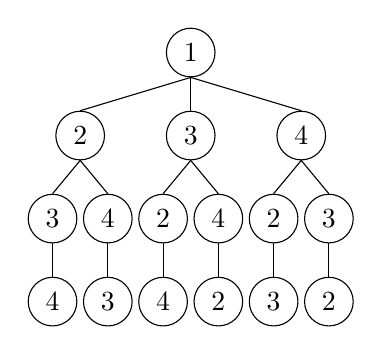
\begin{tikzpicture}[every tree node/.style={draw,circle}]
    \Tree [.\node{1};
            [.\node{2};
                [.\node{3};
                    [.\node{4}; ]
                ]
                [.\node{4};
                    [.\node{3}; ]
                ]
            ]
            [.\node{3};
                [.\node{2};
                    [.\node{4}; ]
                ]
                [.\node{4};
                    [.\node{2}; ]
                ]
            ]
            [.\node{4};
                [.\node{2};
                    [.\node{3}; ]
                ]
                [.\node{3};
                    [.\node{2}; ]
                ]
            ]
        ]
\end{tikzpicture}
\caption{All permutations of $(1,2,3,4)$, with $1$ fixed as the first element, visualized as a decision tree.}
\end{subfigure}
\caption{A pseudocode and visual representation of a recursive enumeration}
\end{figure}

Therefore, version 3 uses recursive enumeration for the tour generation, computing the sub-tour cost on each level, and pruning whenever the partial sum is bigger than the previously known optimum by not recursing deeper.

Analogous to this approach, the next versions will use pruning extensively to achieve better performance by reducing the number of permutations to compute the cost for.

\paragraph{Version 4: Prune using \ac{NN} Metric:}

In version 3, the subgraph was pruned iff it already costs more than the previously known minimum. To prune more aggressively, now a subgraph will be pruned iff its cost plus a lower bound on the remaining vertices is bigger than the current minimum. A graph qualifies as a lower bound if its cumulative cost is below the sum of the costs of the vertices added to the \ac{TSP} solution;

Here, the \acl{NN} lower bound will be used\footnote{Not to be confused with the \acl{NN} algorithm used for approximating a solution.}. The \ac{NN} graph will be computed by connecting each vertex to its nearest neighbour. Note that the resulting graph can have multi-edges and doesn't have to be fully connected.

Let $p$ be our recursively enumerated subpath, $v_1,\dots,v_m$ be the free vertices (i.e. $v_i \not\in p$), and $c : V \times V \rightarrow \mathbb{R}$ be the cost function. The nearest neighbour graph can be computed in $\Theta(m^2)$ using the following formula:


\begin{figure}[H]
\centering
\begin{subfigure}[c]{0.45\textwidth}
\includegraphics[width=\textwidth]{./assets/nn.png}
\caption{} % generates a (a)
\centering
\end{subfigure}
\begin{subfigure}[c]{0.45\textwidth}
\[
c_{NN} := \sum_{i \in \{1,\dots,m\}} \min_{\substack{j \in \{1,\dots,m\}\\ i \neq j}} c(i,j)
\]
\caption{} % generates a (b)
\end{subfigure}
\caption{An example subgraph with a \ac{NN} lower bound (a) and the formal for computing the total cost of an \ac{NN} (b).}
\end{figure}

Note that this is an obvious improvement over the previous lower bound for pruning since $p+c_{NN}$ is a tighter bound than $p+0$.

\paragraph{Version 5: Prune using the \ac{MST} Metric:}

This version uses the same approach as version 4, but instead of computing a \ac{NN} graph, it computes the previously defined \ac{MST} from the remaining vertices. This is an even tighter bound.

\begin{figure}[H]
\centering
\begin{subfigure}[c]{0.45\textwidth}
\includegraphics[width=\textwidth]{./assets/nn.png}
\caption{} % generates a (a)
\centering
\end{subfigure}
\centering
\begin{subfigure}[c]{0.45\textwidth}
\includegraphics[width=\textwidth]{./assets/mst.png}
\caption{} % generates a (b)
\centering
\end{subfigure}
\caption{Comparison between the \ac{NN} (a) and \ac{MST} (b) graph of the remaining vertices for an example graph.}
\end{figure}

Note that it is not obvious that this algorithm will perform better than the previous versions. While it improves its pruning ability, it also adds the cost of computing all \acp{MST}. In the next and last version, those \acp{MST} will be cached to reduce redundant computations.

\paragraph{Version 6: Cache the previous \acp{MST}:}
The last version builds upon version 5, but caches the \acp{MST} so that the amount of redundant compute is reduced. This requires a fast \ac{MST} lookup; in our code a HashMap was used, resulting in $O(1)$ average lookup time. Furthermore, instead of using the default HashMap, a cryptographically insecure but overall more performant HashMap was used \cite{noauthor_rustc-hash_2023}\footnote{As the name implies, \texttt{rustc-hash} is also used in the compiler itself and maintained by the Rust core team.}.

\subsubsection{Prefix Space Partitioning}

For explaining both the shared and distributed parallelization algorithms, the concept of \textbf{prefix space partitioning} is required.

As explained before, a \ac{TSP} solution of an $n$-vertex graph can be viewed as an $n$-dimensional vector. Furthermore, since the paths are generated using recursive enumeration, the prefix of a path can be used to compute all subpaths containing that prefix. This means that the prefixes of a given length form an equivalence relation on the set of all paths. Since all equivalence classes have the same size, one can evenly partition the work by dividing the number of prefixes by the number of workers.

This mapping is archived by interpreting a prefix as a $n$-ary number.

\begin{definition}{Mapping paths to $n$-ary numbers:}
A path $v :=(v_1,\dots,v_m)$ of an $n$-vertex graph can be mapped to a number by interpreting the $i$-th element as the $i$-th digit of an $n$-ary number.
Formally, the mapping function $\rho_{n,m}$ can be defined as
\begin{align*}
    \rho_{n,m} &: \{1,\dots,n\}^m \rightarrow \mathbb{N}\\
    \rho_{n,m}(v_1,\dots,n_m) &:= \sum_{i=1}^m n^{i-1} v_{i}
\end{align*}
Let $\rho_{n,m}^{-1}$ be defined as the inverse, i.e. $\rho_{n,m}^{-1}(\rho_{n,m}(x)) = x$.
\end{definition}

\begin{example}
    This is analogous (but reversed) to how natural numbers in base $10$ can be defined.
    \[
        (12345)_{10} = 5 \cdot 10^0 + 4 \cdot 10^1 + 3 \cdot 10^2 + 2 \cdot 10^3 + 1 \cdot 10^4 = \rho_{10,5}(5,4,3,2,1)
    \]
\end{example}

\begin{example}
    This is also how binary numbers are converted into the decimal system.
    \[
        (10001)_2 = 1 \cdot 2^0 + 1 \cdot 2^4 = 9 = \rho_{2,5}(1,0,0,0,1)
    \]
\end{example}

Now, with this number mapping in mind, the prefix space partitioning algorithm can be properly defined:
\begin{definition}{Prefix Space Partitioning Algorithm:}
    Given a graph with $n$ vertices, a prefix length of $m$ and $p$ workers, the $i$-th worker can compute his prefix range as follows:
\begin{enumerate}
    \item Compute the total number of prefix values, including invalid paths: $n^m$.
    \item Calculate the $i$-th chunk of all path ids: $[l,r) := [n^m/p \cdot (i-1), n^m/p\cdot i)$
    \item Map and return the prefixes associated with those bounds:
        \begin{itemize}
            \item Starting Value: $\rho_{n,m}^{-1}(l)$
            \item Ending Value (exclusive): $\rho_{n,m}^{-1}(r)$
        \end{itemize}
\end{enumerate}
\end{definition}

\begin{remark}
    Note that this prefix space partitioning can be done locally on each worker without any communication needed by using its rank and the world size.
\end{remark}


\subsubsection{Shared Memory Parallelization}

With the idea of prefix space partitioning in mind, the shared memory parallelization algorithm is straightforward:

\begin{enumerate}
\item Start $n$ threads. $n$ can be manually specified, otherwise it defaults to\\\texttt{std::thread::available\_parallelism}.
\item Each thread computes its prefix space using prefix space partitioning.\\
    The prefix length can be manually specified, otherwise it defaults to $3$.
\item Each thread computes each valid tour in its prefix space.
\end{enumerate}

The threads prune using the \ac{MST} lower bound of the version 5 sequential algorithm. The current minimum is potentially updated after every tour. Synchronization is done via a mutex, of which all threads get an atomically counted reference. Note that we do not cache the \acp{MST} as the performance boost was negligible while resulting in a lot of locking.

\subsubsection{Statically Partitioned Distributed Memory Parallelization}

The statically partitioned, \acs{MPI}-based solver works analogously to the multi-threaded version, using both the \acs{MST} lower bound as well as the prefix space partitioning.

This means that it
\begin{itemize}
\item divides up the work through prefix space partitioning.
\item goes through all possible solutions that can't be pruned away.
\item generates all possible paths through recursive enumeration.
\item caches the sum of the partial path throughout the recursion.
\item prunes iff the partial sum plus the \acs{MST} lower bound is bigger than the known optimum.
\end{itemize}

Now to the communication. Let us assume that the communicator world size is $n$. We choose rank $0$ as the communicator and rank $\{1,\dots,n-1\}$ as the workers.

Using prefix space partitioning\footnote{Variadic prefix length, defaults to $3$ vertices.}, each worker knows the prefixes it has to process. In order to prune, every time a worker finishes a prefix, it sends its current lowest cost it ever encountered to the coordinator. This is done even if it was not improved during that prefix.

It is done because this message is also used as an update request for the newest global minimum known from the coordinator. After taking the worker's minimum into account, it returns the global minimum that all workers ever archived. Note that only the cost and not the full path is sent to minimize the amount of traffic between the communicator and the workers. After all assigned prefixes are computed, the worker waits at a barrier for the other workers to complete.

Since the workers prune, the coordinator can not know how many requests it can expect from each worker. Thus, each worker has to tell the coordinator when it is done, otherwise, it will deadlock waiting for yet another processed prefix.

This is done by sending another message with a negative cost. The coordinator tracks how many of those messages were received. Once the coordinator receives $n-1$ messages it stops listening. Receiving $n-1$ finish messages implies that all workers are already waiting at the barrier. Thus, the coordinator joins the barrier node; breaking the barrier and starting the wrapup.

After the barrier was broken, the coordinator broadcasts which rank won with which cost. Therefore, all workers know who won. The winner then finally broadcasts the winning tour to every other node. Thus, in the end, every worker knows the best cost from the coordinator and the best path from the winner. Again, note that the wrapup is a network efficiency optimization since it allowed us to not send the current best path to the coordinator each time it was improved by a worker.

\subsubsection{Dynamically Partitioned Distributed Memory Parallelization}

This algorithm is an optimization of the previous \acs{MPI}-based algorithm. This is only done by changing the communication scheme. Thus, the algorithmic steps are the same as the statically partitioned algorithm.

In the static solver, the load was divided locally through the rank and prefix space partitioning. This is easy to compute since one can just divide with $n$-ary numbers.

But, especially since the problem is factorial, the problem should be pruned as much as possible. In the static version, this was done by telling the root the local minimum it currently knows, and as an answer receiving the global current minimum with that answer in mind. \emph{Note that this requires one bidirectional communication per prefix}.

This approach has one disadvantage. Note that, while the pruning greatly optimizes the average-case scenario, it does not improve the worst-case scenario. The algorithm performs great, but its performance is very dependent on the graph and its pruneability. The same logic applies to all subgraphs with fixed prefixes.

The workers have (potentially) vastly different workloads, depending on how well they can prune. Since the coordinator has to wait for all workers to finish before it knows the global best solution, all finished workers have to idle, wasting precious compute. Even more important, global work coordination wouldn't even increase the amount of communications, since we do one bi-directional send and receive per prefix nonetheless.

Thus, instead of using prefix space partitioning to predivide it statically, the computation workflow is as follows:
\begin{enumerate}
    \item The worker asks the coordinator for a new prefix to compute\footnote{For easier \ac{MPI} communication, prefixes have a fixed length of $3$ vertices.}.
\item The coordinator answers with the next non-computed prefix as well as the current minimum.\\
    If all prefixes are computed, the worker receives a prefix with all zeroes, which means it waits at a barrier for the others to finish.
\item The worker computes the current prefix given to it.\\
    It uses the current global minimum given with the prefix to prune accordingly.
\item The worker returns its local minimum to the work node.\\
    This is an implicit ask for more work.\\
    The root node can use that node-specific minimum to update the global minimum if needed.
\end{enumerate}

Although the root could already know which prefix resulted in the global minimum by keeping track of which ones it assigned to whom, it does not know the whole minimal path. Thus, it needs the same wrapup as the static solver.

After the barrier was broken, the coordinator broadcasts which rank won with which cost. Therefore, all workers know who won. The winner then finally broadcasts the winning tour to every other node. Thus, in the end, every worker knows the best cost from the coordinator and the best path from the winner. Again, note that the wrapup is a network efficiency optimization since it allowed us to not send the current best path to the coordinator each time it was improved by a worker.

\subsection{Approximate Solving}
Walky provides two different approximation algorithms for solving the \ac{TSP}: The \emph{Nearest Neighbour} algorithm, which provides a simple but not tight approximation, and the \emph{Christofides} algorithm, which is more sophisticated but produces a tighter bound.

\subsubsection{Nearest Neighbour}
The 1-nearest-neighbour algorithm\footnote{Not to be confused with the nearest neighbour lower bound used for exact solving.} is a simple, straightforward greedy algorithm to compute an approximation for the \ac{TSP}. It works as follows:

\paragraph{Algorithm:}

\begin{itemize}
\item Choose a random starting node.
\item From that node, greedily visit the nearest node which was not visited before.
\item Repeat until all nodes are visited.
\item Return to the starting node to close the tour.
\end{itemize}

In walky, the nearest neighbour algorithm computes the 1-nearest-neighbour for all starting nodes and returns the minimum. Since the 1-nearest-neighbour has a complexity of $\Theta(n^2)$, the nearest neighbour has a complexity of $\Theta(n^3)$.

\paragraph{Shared-Memory Parallelization:} The parallelization was done trivially. Using the \texttt{rayon} create, all staring nodes were processed parallelly using a preallocated thread pool. The results were then reduced to get the global minimum.

\paragraph{Distributed-Memory Parallelization:} The \acs{MPI}-based implementation uses a simplified version of the aforementioned prefix space partitioning.

This algorithm requires no coordinator, i.e. all nodes are workers. The 1-nearest-neighbour computations will be done sequentially, the parallelization consists of the workload partitioning through the starting nodes.

Given an $n$-vertex graph and $m$ workers, the $i$-th rank computes the 1-nearest-neighbour for the starting nodes $[n/m\cdot i, n/m \cdot (i+1))$. Since every worker knows its rank, this can be computed locally and independently without any communication.

Once the minimum of that local chunk has been found, the \acs{MPI} communication starts. First, through an \texttt{ALL\_REDUCE} on the cost every worker finds out the best cost and which worker won. After that, the best worker knows that it won. It then proceeds to broadcast the whole path to everyone. Analogously to the static exact solver, this is a network efficiency optimization by only sending one path through the network at the end.

Now every worker knows the global minimum and can successfully return it.

\subsubsection{Christofides Algorithm}

Next is an algorithm that requires more assumptions on the input,
but also gives an approximation to the TSP that is guaranteed to have
a weight $\leq 1.5 \cdot \omega$, with $\omega$ being the weight of the optimal solution
\cite{christofides_worst-case_1976}.
The algorithm requires two preliminary definitions.

\begin{definition}[Matching]
  See \cite{weisstein_matching_nodate}.
  Let $G = (V, E)$ be a Graph.
  A set $M \subseteq E$ is called \emph{matching} of $G$, if
  all edges in $M$ are pairwise disjoint
  $$ \forall x,y \in M: x \cap y = \emptyset $$.
  \label{def:matching}
\end{definition}

\begin{definition}[Perfect Matching]
  See \cite{weisstein_matching_nodate}.
  Let $G = (V, E)$ be a graph and $M \subseteq E$ be a matching of $G$.
  Then, $M$ is called \emph{perfect}, if $M$ spans the whole graph
  $$ \forall v \in V \, \exists e \in M: v \in e $$.
  \label{def:perfect_matching}
\end{definition}

Now, the Christofides Algorithm can be defined.

\begin{definition}[Christofides Algorithm]
  Let $G = (V, E)$ be a metric Graph (i.e. the triangle inequality holds).
  The Christofides algorithm is a five-step procedure \cite{christofides_worst-case_1976}:
    \begin{enumerate}
      \item Calculate the \ac{MST} of $G$: \ac{MST} $= (V_{M}, E_{M})$.
      \item Calculate an exact matching in $S:= (E_S, V_S)$.

        Let $V_S := \{v \in V_M | \deg_M(v) \equiv 1 \mod 2\}$ the set of all vertices that have
        odd degree in the \ac{MST}.
        Then let $E_S := \{e \in V_G | e = (e_1, e_2) \wedge e_1 \in V_S \wedge e_2 \in V_S\}$.
        Of all possible perfect matchings, choose one with minimal weight.
      \item Combine the \ac{MST} and the matching into one multigraph.
      \item Find an Eulerian cycle through the multigraph.
      \item Make the Eulerian cycle Hamiltonian.
    \end{enumerate}
    \label{def:christofides}
\end{definition}
\begin{remark}
  According to \cite{christofides_worst-case_1976}, in step 2 a perfect matching
  can always be found.
\end{remark}

Some of the above steps use constructs that are not defined yet. 
Those steps will be elaborated on below.
In contrast to that, for step 1 simply refer to section \ref{sec:mst}.

\paragraph{Explaining Step 2 Of Christofides Algorithm}

In definition \ref{def:christofides}, only a high-level description for step 2 was provided.
To provide further explanation, a visualization of that step on the $K_5$ graph follows.

Let $G = K_5$. Edge weights are left out for the simplicity of visualization.
In the left graph,
an \ac{MST} of $G$ is highlighted with bold edges in black.
The vertices of odd degree w.r.t the MST are: $1,2,3,4$.
The task is then to find a matching over these vertices.
The resulting matching is visualized in the right graph with blue edges.

\begin{minipage}{0.45\textwidth}
  \centering
  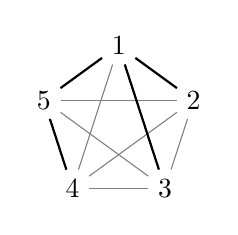
\begin{tikzpicture}
    \graph { subgraph K_n [n=5, clockwise, edges=gray];
      (1) --[thick] (2);
      (1) --[thick] (5);
      (5) --[thick] (4);
      (1) --[thick] (3); };
    
  \end{tikzpicture}
\end{minipage}
\hfill
\begin{minipage}{0.45\textwidth}
  \centering
  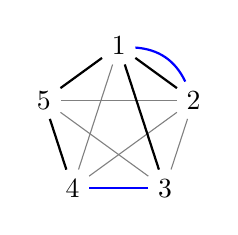
\begin{tikzpicture}
    \graph { subgraph K_n [n=5, clockwise, edges=gray];
      (1) --[thick] (2);
      (1) --[thick] (5);
      (5) --[thick] (4);
      (1) --[thick] (3);
      (4) --[thick, blue] (3);
      (1) --[thick, blue, bend left] (2);
    };
  \end{tikzpicture}

\end{minipage}

\paragraph{Finding A Matching}
Executing the Christofides Algorithm involves finding a minimum-cost perfect matching.
In a sequential setting Edmonds's Blossom Algorithm\footnote{For a definition and live demonstration see
\url{https://algorithms.discrete.ma.tum.de/graph-algorithms/matchings-blossom-algorithm/index_en.html}.}
gives an exact solution to the problem.
Instead of this algorithm, a na\"ive randomized approximate solution was implemented,
to be able to utilize parallelization.

The randomized approximate solution follows this idea:
randomly guess a matching and do some randomized improvements.
Repeat this and take the matching with minimal cost.
This solution is easy to implement and easy to parallelize.

\begin{definition}[Algorithm: Finding an initial matching]
  Let $G = (V,E)$ be a complete graph with an even amount of vertices
  $|V| = 2n, n \in \NN$. W.l.o.g. let $V = \{1,\dots,2n\}$.
  Select a permutation $\pi: V \rightarrow V$ uniformly at random.
  Now $$M = \{\{\pi(1), \pi(2)\}, \dots, \{\pi(2n-1), \pi(2n)\}\}$$
  is a perfect matching of $G$.
  \label{algo:rand_matching}
\end{definition}


Now, focus on improving a matching consisting of only 2 edges.
\begin{theorem}[Minimum-cost perfect matching on $K_4$]
  Given the Graph $K_4 = (V,E)$
  w.o.l.g. $V = \{\{1,2\},\{3,4\}\}$.
  Then exactly 3 perfect matchings exist on $K_4$:

  \vspace{0.5\baselineskip}
  \hfill
  \begin{tikzpicture}
    \node (1) at (0,1) {1};
    \node (2) at (0,0) {2};
    \node (3) at (1,1) {3};
    \node (4) at (1,0) {4};
    \graph { (1) -- (2); (3) -- (4)  };
  \end{tikzpicture}, \hfill
  \begin{tikzpicture}
    \node (1) at (0,1) {1};
    \node (2) at (0,0) {2};
    \node (3) at (1,1) {3};
    \node (4) at (1,0) {4};
    \graph { (1) -- (3); (2) -- (4)  };
  \end{tikzpicture}, \hfill
  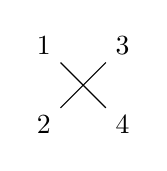
\begin{tikzpicture}
    \node (1) at (0,1) {1};
    \node (2) at (0,0) {2};
    \node (3) at (1,1) {3};
    \node (4) at (1,0) {4};
    \graph { (1) -- (4); (2) -- (3)  };
  \end{tikzpicture}
  \hspace{0.2\textwidth}
  \vspace{0.5\baselineskip}
 

  A matching with the lowest cost is a minimum-cost perfect matching on $K_4$.
  \label{thm:perfect_matching_k4}
\end{theorem}
\begin{proof}
  When constructing a matching for $K_4$, there are ${4 \choose 2} = 6$
  options for the first edge $e_1 = \{a,b\}$. The choice for the second edge immediately follows
  as $e_2 = \{c,d\}$, by the property of a matching: $e_1 \cap e_2 = \emptyset$.
  Then $M = \{e_1, e_2\}$. Because the order of edges is unimportant for the matching,
  for every choice of $(e_1, e_2)$, there is one choice $(e_1', e_2')$ with
  $e_1 = e_2' \wedge e_2 = e_1'$.
  Therefore, there are $\frac{6}{2} = 3$ perfect matchings on $K_4$.
\end{proof}

With this theorem, one can improve matchings of arbitrary size.

\begin{definition}[Randomly Improving A Matching]
  Let $$M = \{m_0,\dots, m_{n-1}\}$$ be a perfect matching on $K_n$, $n \in \NN$.
  Repeat the following procedure $k \in \NN$ times:

  Uniformly at random select a permutation $\pi: M \rightarrow M$.
  For every perfect matching
  \begin{align*}
    &M_i' = \{\pi(m_{2i}), \pi(m_{2i+1})\}, &i = 0,\dots, \left\lfloor{\frac{n}{2}}\right\rfloor&
  \end{align*}
  on the corresponding subgraph $K' \subseteq K_n$ with $K' \cong K_4$,
  use theorem \ref{thm:perfect_matching_k4} to compute a minimum-cost perfect matching $\widetilde{M_i'}$.
  Then set
  $$
  M \leftarrow \left\{\widetilde{M_i'} | i \in \left\{i = 0,\dots, \left\lfloor{\frac{n}{2}}\right\rfloor\right\}\right\}
    \cup \begin{cases} \{\pi(m_{n-1})\}&, \text{ if } n \text{ is odd} \\ \emptyset &,\text{ else}\end{cases}
  $$.
  \label{algo:random_matching_improvement}
\end{definition}
\begin{remark}
  The application of theorem \ref{thm:perfect_matching_k4} on each $M_i'$ can be parallelized,
  as the computation for each $i$ is independent of all other computations.
\end{remark}


\paragraph{Last Steps Of Christofides Algorithm}
For step 4 one needs to compute an Eulerian cycle. This is done with an implementation of
Hierholzer's algorithm \cite{hierholzer_ueber_1873}\cite[Algorithm X.4]{fleischner_algorithms_1991}.


Finally, step 5 is easily done using the metric property of the complete input graph: 
Start the Hamiltonian cycle at some vertex and keep track of which vertices have been visited
while traversing the Eulerian cycle.
If a vertex has not been visited, add it to the Hamiltonian cycle.
If a vertex has already been visited, simply skip it and proceed with the next vertex.
Such shortcuts exist because the graph is complete,
and taking these shortcuts does not increase the weight of the solution, since 
the graph is metric whereby the triangle inequality holds.

\paragraph{Parallelization}
\label{paragraph:christofides_mpi}
There is a parallel implementation using rayon, and one using \ac{MPI}.
Both only parallelize the improvement of randomized matchings, as in Def. \ref{algo:random_matching_improvement}.

The shared memory implementation distributes all the consecutive pairs of edges
between the available threads, and computes the improved 2-matchings (see Def. \ref{thm:perfect_matching_k4}) in parallel.
Then, a new matching is constructed from all partial values of the threads.
The details of synchronization and message passing are handled by the rayon \texttt{ParallelIterator} implementation.

The \ac{MPI}-based parallelization uses a different approach:
The randomized improvement of the matching is done independently at each process,
only at the end the results are gathered at the root process
and the matching with the least cost is chosen. For this,
each process sends the local solution and the corresponding solution weight
to the root process per \ac{MPI} unicast. This is not optimal,
as the optimal solution weight could be determined by a global reduction,
such that only one full solution vector would need to be sent.
Because the Rust \ac{MPI} interface
\texttt{rsmpi}\footnote{This will be introduced in more detail in section \ref{sec:parallelism_libraries}.}
does not support the
\texttt{MPI\_MAXLOC}\footnote{For a description of the operation see
  \cite[section 5.9.4]{message_passing_interface_forum_mpi_2015}.}
operation at the moment, but the location of the maximum weight is needed,
a simple reduction would not suffice.


\subsection{Lower Bound}

So far, there are multiple techniques for approximation a solution to the \ac{TSP},
each result provides an upper bound on the exact solution.
Now comes a brief look at computing lower bounds to the \ac{TSP}.

\subsubsection{MST Lower Bound}

The \ac{MST} of a graph is, in comparison to the \ac{TSP}, fairly easy to compute.
It turns out, that the \ac{MST} provides a lower bound to the \ac{TSP} in a very natural way.

\begin{theorem}[MST lower bound]
  Let $G$ be a weighted, complete graph. Let $T_G$ be an exact solution to the \ac{TSP} on $G$,
  with weight $w_T$.
  Let $M$ be an \ac{MST} of $G$, with weight $w_M$.
  Then $$w_M \leq w_T$$ holds.
  \label{thm:mst_lower_bound}
\end{theorem}
\begin{proof}
  $T$ is the solution to the \ac{TSP} on $G$. By definition, $T$ then is an Eulerian cycle,
  that visits each vertex in $G$ exactly once.
  Therefore, by removing any edge from $T$, one yields a spanning tree $S$ of $G$, with weight $w_S$.
  By definition, $$w_M \leq w_S \leq w_T$$ follows.
\end{proof}

\subsubsection{1-tree Lower Bound}
\label{sec:1-tree}

One can improve upon the \ac{MST}-based approach,
by using a variation of the \ac{MST}, called minimum-weight 1-tree.

\begin{definition}[1-tree]
  See \cite[p. 1139]{held_traveling-salesman_1970}.
  Let $G=(V,E)$ be a graph.
  Let $\{v_1,\dots,v_n\} = V$ be some enumeration of all vertices $V$.
  Then a 1-tree on $G$ is defined to be
  \begin{enumerate}
    \item a tree, when restricted to the vertices $\{v_2,\dots,v_n\}$,
    \item and to have exactly one cycle. This cycle goes through vertex $v_1$.
  \end{enumerate}
  \label{def:1_tree}
\end{definition}

In the extreme case, such a 1-tree can be a cycle in a graph.

\begin{theorem}[Cycle as a 1-tree]
  Let $G$ be a Graph, and $C$ be a circle in $G$.
  The $C$ is a 1-tree.
  \label{thm:cycle_is_1_tree}
\end{theorem}
\begin{proof}
  Let $G = (V,E)$, and let $V = \{v_1, \dots, v_n\}$ be some enumeration.
    Then $C|_{\{v_2,\dots,v_n\}}$ is a tree. By definition, $C$ contains exactly one cycle,
    and it goes through $v_1$. Therefore, all properties of Def. \ref{def:1_tree} apply to $C$.
\end{proof}

The 1-trees for the lower bound must also be of minimal weight.

\begin{definition}[minimum-weight 1-tree]
  See \cite[p. 1139]{held_traveling-salesman_1970}.
  Let $G=(V,E)$ be a weighted graph.
  Let $\{v_1,\dots,v_n\} = V$ be some enumeration of all vertices $V$.
  Then a minimum-weight 1-tree on $G$ is a 1-tree, that also is
  \begin{enumerate}
    \item an \ac{MST} when restricted to the vertices $\{v_2,\dots,v_n\}$,
    \item and the special vertex $v_1$ is connected to the rest of the 1-tree with
      the two distinct cheapest edges.
  \end{enumerate}
  \label{def:min_weight_1_tree}
\end{definition}
\begin{remark}
  For every choice of the special vertex $v_1$, there is a possibly distinct minimum-weight 1-tree.
  All of these 1-trees can be computed independently of each other, which is easy to parallelize.
  This point will be revisited later.
\end{remark}


Combining this knowledge, one can now construct a tighter lower bound on the \ac{TSP}.
\begin{theorem}[1-tree lower bound]
  Let $G$ be a weighted, complete graph. Let $T_G$ be an exact solution to the \ac{TSP} on $G$,
  with weight $w_T$.
  Let $\mathcal{M}$ be the set of all minimum-weight 1-trees of $G$,
  and let $W_\mathcal{M}$ be the set of the corresponding weights.
  Then $$\max_{w_M \in W_\mathcal{M}}w_M \leq w_T$$ holds.
  \label{thm:1_tree_lower_bound}
\end{theorem}
\begin{proof}
  Let $M \in \mathcal{M}$ with weight $w_m$, s.t. $$w_M = \max_{w \in W_\mathcal{M}}w$$.
  Then, let $v_1$ be the special vertex of $M$.
  $T$ is an Eulerian cycle, thus by Theorem \ref{thm:cycle_is_1_tree} it is a 1-tree on $G$,
  with special vertex $v_1$.
  Since $M$ has minimal weight, $$w_M \leq w_T$$ follows immediately.
\end{proof}
\begin{remark}
  When removing one edge incident to the special vertex $v_1$ from a 1-tree, one yields a spanning tree.
  Thus, the 1-tree lower bound is tighter than the \ac{MST} lower bound.
\end{remark}

The sequential implementation is straightforward and
follows directly from the above-mentioned definitions.
It leverages the fact, that the used implementation of Prim's algorithm
is capable of ignoring one vertex in a given graph,
which is then used to construct the 1-trees.

There are two parallel implementations provided, one using rayon, and one using \ac{MPI}.

For rayon, the parallelization is again handled by the \texttt{ParallelIterator} implementation.
For every vertex in the graph there is a minimum-weight 1-tree (see Def. \ref{def:min_weight_1_tree}).
In principle, these 1-trees can be computed in separate threads. At the end, the maximum of the
tree weights is computed over all threads.

The \ac{MPI} version follows the same idea. Each process knows their rank $r$ and the size $s$ of the \ac{MPI} world.
Then, the process computes a minimum-weight 1-tree for each vertex $u$,
where $u \equiv r \mod s$.
Afterwards, using an \ac{MPI} reduction, the maximum over all processes is collected at the root process.

\newpage

\section{Implementation}

\subsection{Rust}
% - Rust introduction from other paper
Rust \cite{noauthor_rust_nodate} is a systems programming language initially released by Mozilla Research in 2015. It was designed as a memory-safe alternative for C++ in Servo \cite{developers_servo_nodate}, which is the web rendering engine used in Firefox. Rust's main goal is to provide memory safety while having an on-par performance with other systems languages such as C or C++. Having memory safety is paramount; research suggests that in memory-unsafe languages, at least 65\% of the security vulnerabilities are caused by memory unsafety. This was discovered simultaneously at Android \cite{stepanov_detecting_2020} \cite{stoep_queue_2019}, iOS and macOS \cite{kehrer_memory_2019}, Chrome \cite{noauthor_memory_nodate}, Microsoft \cite{thomas_proactive_2019}, Firefox \cite{hosfelt_implications_2019}, and Ubuntu \cite{geoffrey_thomas_geofft_unofficial_2019}.

Specifically, Rust is great for \ac{HPC} since one can think of it as a modern dialect of C++ enforced by the compiler. It uses \acs{RAII}\footnote{\acf{RAII}} internally to ensure memory safety, while references are roughly equivalent to \texttt{std::unique\_ptr}. While Rust's ecosystem itself is still maturing, due to its clean \ac{FFI} and simple bidirectional C++ \cite{you_bindgen_2023} and Python \cite{pyo3_project_and_contributors_pyo3_2023} interoperability allows for seamless integration into a typical \ac{HPC} environment. Analogously, while the Rust compiler is comparatively new, it already supports most compiler optimizations by leveraging \ac{LLVM} as a compiler backend. It is natively compiled without a garbage collector.

Lastly, with its many functional patterns, it is a very loved language by the industry and developers alike. According to the yearly StackOverflow survey it was voted as the most loved language for the 7th year in a row \cite{noauthor_stack_2023}. It rapidly gets adopted by big tech firms such as AWS \cite{asay_why_2020}, Google \cite{noauthor_welcome_nodate}, Meta \cite{garcia_programming_2022}, and Microsoft \cite{jirehl_microsoft_2022} and is even accepted as a language for the Linux kernel \cite{claburn_linus_2022}.

Walky requires an \ac{MSRV} of 1.70.0\footnote{This does not require that 1.70.0 or higher is available as a cluster module because Rust uses \texttt{rustup} \cite{noauthor_rustuprs_nodate} for easy userspace installation management.}. Since \ac{MPI} support is hidden behind a feature flag, no \ac{MPI} is required for compilation.


\subsection{Compiler Optimizations}
To ensure the best possible performance, the following compiler optimizations were explicitly enabled:
\begin{itemize}
  \item \textbf{Release Builds (\texttt{-O3})}: If one does not use the release build\footnote{With \texttt{cargo build \textemdash\textemdash release}.} the code is not optimized. This enables several general optimizations as well as automatic vectorization.
  \item \textbf{\ac{LLVM} \ac{LTO}}: \ac{LTO} enabled further, intermodular optimizations during the link stage. While this could improve code by optimizing beyond library bounds, it increases compile time, which is why it is disabled by default.
  \item \textbf{Compiling for Native Architecture:} When compiling for the native architecture\footnote{Using the \texttt{RUSTFLAGS} environment variable, i.e. \texttt{RUSTFLAGS="-C target-cpu=native" cargo build \textemdash\textemdash release}.} the compiler can use more specialized instructions that are not available on every processor such as bigger vector registers for SIMD. Note that this may create binaries incompatible with other systems.
  \item \textbf{Using a single \ac{LLVM} codegen unit:} Codegen units are analogous to translation units. This means that, when changing a single file, just the codegen unit in that file has to be recompiled. Therefore, optimizations can't be done beyond codegen unit bounds! Using a single codegen for the whole project allows the compiler to more aggressively optimize globally. Note that this effectively disables partial compilations.
\end{itemize}

\subsection{Command Line Interface (CLI)}

The \texttt{walky} binary implements a \ac{CLI} using the crate \href{https://crates.io/crates/clap}{\texttt{clap}},
structured with subcommands.

For the following demonstration of the \ac{CLI},
the \texttt{walky} binary has been compiled with
\begin{minted}[breaklines, fontsize=\footnotesize]{text}
$ cargo build --release --features mpi
\end{minted}

\texttt{walky} displays an overview of its subcommands:
\begin{minted}[breaklines, fontsize=\footnotesize]{text}
$ walky --help
A TSP solver written in Rust

Usage: walky <COMMAND>

Commands:
  exact        Find the exact best solution to a given TSP instance
  approx       Find an approximate solution to a given TSP instance
  lower-bound  Compute a lower bound cost of a TSP instance
  help         Print this message or the help of the given subcommand(s)

Options:
  -h, --help     Print help
  -V, --version  Print version
\end{minted}

Each subcommand follows the same basic syntax.

\begin{minted}[fontsize=\footnotesize]{text}
walky SUBCOMMAND [OPTIONS] <ALGORITHM> <INPUT_FILE>
\end{minted}

Users need to specify a subcommand. Then, they can provide optional parameters, after which
they need to specify a concrete algorithm to use and a file path to the input file.
The full help for every subcommand is listed in section \ref{sec:walky_subcommands}.

\subsection{Parallelism Libraries}
\label{sec:parallelism_libraries}
For both shared- and distributed memory parallelism, specialized Rust crates were used:

\paragraph{Shared Memory Parallelism:} For shared memory parallelism we used the rayon \cite{noauthor_rayon_2023} crate. Rayon is a high-level parallelism library using dynamically sized thread pools. It guarantees \emph{data-race freedom} by allowing only one thread to write at a time. Its main features are drop-in parallel iterators: By replacing \texttt{.iter()} with \texttt{.par\_iter}, it is possible to use all functions provided for iterators, such as \texttt{.map()}, \texttt{.filter()}, \texttt{.reduce()} for typical functional patterns or \texttt{.join(|| a(), || b())} enabling the \texttt{fork-join} computation model. Thus, when initially written in an iterator-focused, functional way it allowed easy parallelization of the previously designed sequential algorithms.

\paragraph{Distributed Memory Parallelism:} For distributed memory, multi-node parallelism the \ac{HPC} native \ac{MPI} environment was leveraged using the rsmpi crate \cite{noauthor_mpi_2023}. rsmpi is a Rust-native \ac{MPI} implementation\footnote{With \ac{FFI} bindings to other implementations through the beforementioned bindgen.} compliant with MPI-3.1. It is tested to be compatible with OpenMPI, MPICH, and MS-MPI for Windows. It supports most \ac{MPI} features, such as blocking and non-blocking point-to-point communication, and most collective communications such as broadcasts or scatter/gather as well as aggregations such as reductions.

\subsection{Correctness and Tests}
To ensure the algorithm's correctness, both tests and runtime precondition checks were implemented:

\paragraph{Testing:} Traditional testing was done using the \texttt{cargo-nextest} \cite{noauthor_nextest_2023} for parallelized unit tests. The algorithms were tested using pre-computed examples\footnote{Note that the Python tooling for the test case generation can still be found in \texttt{./utils} in the walky repository}, working as follows:

\begin{enumerate}
\item Generate a metric, fully connected, undirected graph by placing $n$ 2D points onto a space and calculating their pairwise distance. This ensures the triangle inequality.
\item Solve the \ac{TSP} for the graph using Python's battle-tested \texttt{python-tsp} \cite{goulart_python_2023}.
\item Generate the input and output Rust code for the test cases using Python.
\end{enumerate}

\paragraph{Preconditions:} At runtime, the following preconditions are checked at runtime before any algorithm starts to ensure correctness:

\begin{itemize}
\item \textbf{Fully Connected:} The \ac{TSP} is only defined for fully connected graphs, i.e. every node has a connection to any other node. This is always true for any real-world examples with metric spaces.
\item \textbf{Undirectedness:} The \ac{TSP} is also only defined for undirected graphs. This means that both directions of an edge should have the same cost, i.e. for any two vertices $A, B$ the edge from $A$ to $B$ should have the same cost as the edge from $B$ to $A$.
\item \textbf{No Multiedges:} Lastly, we require that no multi-edges exist. This means that for any two edges $A$ and $B$, there exists only one direct connection.
\end{itemize}

\subsection{\ac{CI} pipeline}
Furthermore, to keep the code quality high, a sophisticated \ac{CI} pipeline was created, running on each commit on \texttt{main} as well as any pull request. It consists of the following steps running in parallel:
\begin{itemize}
\item \textbf{Build:} First and foremost, it is checked that the current version builds with release settings using \texttt{cargo build}. Note that, due to the limited Ubuntu \ac{CI} runner, the \ac{MPI} feature is disabled.
\item \textbf{Tests:} Next, the automated unit tests are run using the aforementioned \texttt{cargo nextest}.
\item \textbf{Formatter:} After that, the code formatting is verified using \texttt{cargo fmt}. The default Rust standard formatting is used.
\item \textbf{Linter:} Also, the general linter \texttt{cargo clippy} is run to prevent common mistakes and ideomatize walky.
\item \textbf{Documentation Linter:} Lastly, \texttt{cargo doc} is used to verify and lint our docstring documentation, on which our HTML-based documentation is based.
\end{itemize}

\subsection{Documentation and Releases}
Lastly, to improve the \ac{UX} for walky, complete documentation and release management were set in place. Walky uses Semantic Versioning. When releasing a new version, the following artifacts become available:
\begin{itemize}
\item \textbf{Registry Upload:} The source code becomes available at \url{crates.io}, which is the default Rust crate registry. This results in being able to install walky using \texttt{cargo install walky}.
\item \textbf{Hosted HTML-Documentation:} Whenever releasing a new version onto \url{crates.io}, an up-to-date, full test searchable HTML documentation becomes available at \url{docs.rs}\footnote{For walky: \url{https://docs.rs/walky/latest/walky/}}.
\end{itemize}

\newpage

\section{Performance Analysis / Evaluation}

In this section, a performance analysis is done on all algorithms implemented in walky. Where applicable, problem size scaling, strong scaling, and \ac{MPI} scaling analysis are done per algorithm. With problem size scaling, the problem size is increased with a fixed amount of parallelism while with strong scaling, the parallelism is increased with a fixed problem size. Due to the missing Score-P support for LLVM and especially cargo, the \ac{MPI} analysis was done purely mathematically.
\subsection{Cluster Setup}

The benchmarks were done on the \ac{SCC} at GWDG, the joint data center of Max Planck Society for the Advancement of Science (MPG) and University of Göttingen.\footnote{\href{https://gwdg.de/en/hpc/systems/scc/}{\url{https://gwdg.de/en/hpc/systems/scc/}}}. The \ac{SCC} is a large \ac{HPC} system, consisting of about 410 compute nodes with over 18000 CPU cores, 99TB RAM, and 5.2 PiB of storage, split into two filesystems.
For our benchmarks, the so-called \texttt{amp} node type, of which 96 exist at the \ac{SCC}, was used. An \texttt{amp} node has two Xeon Platinum 9242 with a total of 48 CPU cores running at a frequency of 3.8 GHz. Each node has 384 GB of RAM. The jobs were assigned using the internal SLURM workload manager.

\subsection{Vampir-based Analysis of Rust \acs{MPI} Code}

It was initially planned to do the distributed analysis of the \ac{MPI} code using Vampir \cite{noauthor_vampir_nodate}.
Vampir internally uses Score-P \cite{brunst_score-p_2012} for the generation of trace log files. 

Unfortunately, Score-P is not supported by the Rust compiler.
While there is literature to show that Score-P can be integrated into the \acs{LLVM} ecosystem \cite{tschuter_llvm_2017}, the source code was never released.
Furthermore, what makes matters worse is that, even if the tool were published, it is still not trivial to include it into
the cargo build process, which is required for building our third-party dependencies\footnote{As many modern languages do, 
Rust does not specify an \ac{ABI} and instead recompiles all subdependencies (for bounds, the C 
\ac{FFI} convention is usually used). This means, that one can't just link against system-wide libraries as in C.}.

Note that this problem is not just contained to Vampir. Other common analysis tools such as Scalasca \cite{noauthor_scalasca_nodate} or TAU \cite{noauthor_tau_nodate} also rely on Score-P internally.

Therefore, the \ac{MPI} analysis will be theoretically by mathematically scaling the number of messages and bytes sent as well 
as their temporal relationship.

\subsection{Exact Solving Benchmarks}

\subsubsection{Problem Size Scaling}

All single threaded iterations of the algorithm, together with the rayon-based multithreaded version with 24 threads, were run for 24h on the cluster, sequentially computing a random graph from size 3 to size 50. Here are the results:
\begin{figure}[H]
    \centering
\includegraphics[width=0.8\textwidth]{./assets/exact-stmt1.pdf}
\caption{} % generates a (a)
    \caption{The results of the exact solver. shows all algorithms until the NN prune}
\end{figure}

\begin{figure}[H]
    \centering
\includegraphics[width=0.8\textwidth]{./assets/exact-stmt.pdf}
\caption{} % generates a (a)
    \caption{The results of the exact solver. shows all algorithms with a smaller $y$-axis}
\end{figure}

For the full results see Table \ref{tab:exact_benchmarks} in the appendix.

The most important insight is that pruning, especially \acs{MST}-based pruning, immensely improves the viability of exact solving. While $n=14$ took over $20$ minutes with the na\"ive version, it was computed in around $0.11$ seconds using the optimized pruner. It was possible to compute $n=50$ in around $0.3$ seconds\footnote{The benchmark was stopped at $n=50$.}.

Other important insights include the following:
\begin{itemize}
    \item The prefix sum caching was even slower than the na\"ive implementation! This was because we changed from the fast iterative permutation algorithm to recursive enumeration. There are several reasons why this is such slow, from function call overhead to less compiler optimization opportunities to not being tail call optimized. But by the time na\"ive pruning was used, it already consistently outperformed the initial $v0$ on the randomly generated graphs.
    \item While pruning generally improves performance, it does not improve performance deterministically, which is shown in the spikes on less-prunable graphs.
    \item The \ac{MST} performance is insanely good. Remember that this is still an $\mathcal{O}(n!)$ worse case algorithm.
    \item The caching did not improve the previous algorithm enough to justify the added complexity. In fact, depending on the graph, it could worsen overall performance.
\end{itemize}

Last but not least, the multithreaded version performed way worse than the sequential one it was based upon. There are several possible reasons for this behaviour: \label{rayondoof}
\begin{itemize}
    \item Context-switching and threading overhead caused by the operating system.
    \item Blocking inter-thread locking on the current best solution, which was in a mutex that every thread got an atomically reference counted pointer for.
    \item Worse cache utilization. The more threads run on the system, the more context switching. Every time the thread is switched, the CPU caches are flushed by the previous program. Furthermore, hyperthreading always at least halves the cache if not destroys it completely by two threads greedily competing for it.
\end{itemize}

\subsubsection{Strong Scaling}

The strong scaling analysis of the \ac{MPI}-based, distributed exact solver requires a more sophisticated analysis. Before looking at the plotted data, let us compare the statically allocated (V0) algorithm to the dynamically allocated (V1) algorithm:

\begin{table}[H]
\centering
    \begin{tabular}{|c|c|c|c|c|c|c|c|}
        \hline
        Type & Total Worker & V0 $\mu$ & V0 $\sigma$ & V0 Efficiency & V1 $\mu$ & V1 $\sigma$ & V1 Efficiency\\
        \hline
        1n2p & 2 & 815.612 & 0.485 & 72.093 & 134.508 & 0.062 & 437.148\\
        2n1p & 2 & 815.850 & 0.453 & 72.072 & 134.787 & 0.091 & 436.245\\
        1n4p & 4 & 750.874 & 1.011 & 39.154 & 100.460 & 9.940 & 292.654\\
        4n1p & 4 & 746.932 & 0.678 & 39.361 & 63.301 & 0.077 & 464.451\\
        8n1p & 8 & 19.223 & 0.075 & 764.690 & 38.952 & 0.069 & 377.388\\
        1n8p & 8 & 19.401 & 0.013 & 757.705 & 39.311 & 0.683 & 373.945\\
        1n16p & 16 & 11.364 & 0.022 & 646.768 & 54.570 & 0.654 & 134.691\\
        2n16p & 32 & 50.456 & 0.534 & 72.836 & 70.250 & 0.566 & 52.313\\
        4n16p & 64 & 989.302 & 1.536 & 1.857 & 81.203 & 0.458 & 22.628\\
        \hline
    \end{tabular}
    \caption{The results of the exact \ac{MPI} solver. Efficiency is computed as prefixes per worker per second. The type $\alpha$n$\beta$p stands for $\alpha$ computing nodes with $\beta$ workers per node.}
\end{table}

As we can see, the worker topology of the \ac{MPI} processes did not change performance significantly. Thus using the smallest mean for any total worker size, we get the following results:

\begin{figure}[H]
  \centering
  \includegraphics[width=0.8\textwidth]{./assets/exact-mpi.pdf}
  \caption{The comparison of the statically and dynamically allocated algorithm for different numbers of workers.}
\end{figure}

One can see that, averaged over all worker sizes, the dynamically partitioned algorithm performed better. This shows that, although more bits are sent, the more efficient allocation is worth the communication overhead. Furthermore, it is expected that the dynamically distributed algorithm performs comparatively better with more vertices, as more vertices increase the likelihood of an unfair static partitioning.

The optimal performance was recorded with the statically partitioned algorithm with 16 workers. Beyond 16 workers, the single coordinator becomes overwhelmed, resulting in longer waiting times for each worker to report their newly solved prefix.

Overall, it can be concluded that for smaller problems, the statically partitioned \ac{MPI} algorithm should be used, while for large graphs and more workers, the dynamically partitioned algorithm is preferred.

\subsubsection{MPI Analysis}

The \ac{MPI} analysis will be split into the statically partitioned and dynamically partitioned algorithm:

\paragraph{Statically partitioned}

Let $m$ be the number of workers, $n$ be the number of vertices in the graph, and $k$ the length of the prefix. Thus, including prefixes that do not form a proper subtour, we have 
\[
    n \cdot (n-1) \cdot (n-2) \cdot \dots \cdot (n-k) = \prod_{i=n-k}^n i
\]
prefixes. No communication is required for the prefix division. After each prefix, the worker sends $128$ bits\footnote{Assuming normal memory alignment.} to the coordinator and receives the global maximum back. Thus, excluding \ac{MPI} overhead, a total of $256 \cdot \prod_{i=n-k}^n i$ bits of data are sent in the actual computation. In the wrap-up, two broadcasts to $m-1$ nodes are done. But since those do not scale with $n$, they can be ignored in the overall complexity.

\paragraph{Dynamically partitioned}
Let $m$ be the number of workers and $n$ be the number of vertices. The prefix length is fixed to $3$. Thus, we have $n\cdot(n-1)\cdot(n-2) := n_{p}$ prefixes.

Each prefix gets assigned to a worker once, together with the current lowest minimum, resulting in $3\cdot64+64=256$ bits of data per message. For each prefix message to be sent, they have to be requested first. A request implicitly sends its rank and the current minimal path, thus $2\cdot64=128$ bits. Therefore, for the actual computation, a total of $n_p \cdot (128+256)$ bits are sent. Like with the statically partitioned solver, the wrap-up cost is independent of the graph size, and can therefore be ignored asymptotically.

\subsection{Nearest Neighbour benchmarks}

\subsubsection{Problem Size Scaling}
To compare the single-node sequential algorithm to the multithreaded version, starting at $n=100$, the graph size was increased in steps of $100$ up to $3000$. The results are as follows:

\begin{figure}[H]
  \centering
  \includegraphics[width=0.8\textwidth]{./assets/nn-stmt.pdf}
  \caption{Problem Size scaling of the Nearest Neighbour algorithm}
\end{figure}

As one can see, in the beginning, the multithreading overhead keeps the problems performing more equally. Furthermore, while the multithreading is properly used, both algorithms keep the same asymptotic complexity. Overall, the nearest neighbour algorithm greatly benefits from multithreading. This was expected, as no inter-thread communication is required for computing the 1-nearest-neighbours. Furthermore, the minimum reduction at the end is single threaded in both versions, resulting in no overhead in the wrap-up.

\subsubsection{Strong Scaling}

For the \ac{MPI} analysis, a strong scaling benchmark was used, with a fixed graph size of $n=3000$. 

\begin{figure}[H]
  \centering
  \includegraphics[width=0.8\textwidth]{./assets/NN-mpi.pdf}
  \caption{Strong scaling of the Nearest Neighbour algorithm}
\end{figure}

As one can see, the algorithm scales well with the amount of nodes. Analogously to the multithreading version, this was expected, as no inter-node communication is required for computing the single 1-nearest-neighbours. Furthermore, since the work partitioning is done locally on each node, no communication is needed for that either. Thus, with only two collective communications at all, \ac{MPI} provides very little overhead.

\subsubsection{MPI Analysis}
Let $m$ be the number of workers and $n$ be the number of vertices.

Since the actual computation does not require any communication, only the wrap-up sends any data at all, by first \texttt{ALL\_REDUCE} the best cost. After that, the best worker broadcasts the whole path. As the implementation of reductions is \ac{MPI}-dependent, it can only be assumed that an \texttt{ALL\_REDUCE} at most sends $m^2$ messages. Since it only sends the current best cost and its rank, it doesn't scale with the number of vertices and can therefore be ignored.

The broadcast at the end probably uses a tree structure internally, thus resulting in $n\cdot64+64$ bits being sent in $\log(m)$ time steps. Therefore, the communication scales linearly in the number of graph vertices.

\subsection{Christofides benchmarks}
\label{sec:christofides_bench}

\subsubsection{Problem Size Scaling}

\begin{figure}[H]
  \centering
  \includegraphics[width=\textwidth]{christofides-stmt.pdf}
  \caption{Problem Size scaling of the Christofides algorithm}
  \label{fig:weak_scaling_christofides}
\end{figure}
To compare the performance between the single-threaded implementation,
and the rayon-based implementation of the 1-tree lower bound,
a problem size scaling analysis is used.

In Figure \ref{fig:weak_scaling_christofides}, one can see that
the single-threaded implementation has roughly cubic
time complexity, w.r.t. the number of nodes in the input graph.

For the tested graph sizes, the multithreaded implementation
has no performance advantage, even the opposite is the case.
The rayon-based implementation has a worse runtime behaviour on all
tested graphs. Note, that the relative penalty diminishes
for larger graphs. For the reasoning, see the analogous problem in \ref{rayondoof}.

\subsubsection{Strong Scaling}

\begin{figure}[H]
  \centering
  \includegraphics[width=\textwidth]{christofides-mpi.pdf}
  \caption{Strong scaling of the Christofides algorithm}
  \label{fig:strong_scaling_christofides}
\end{figure}

To assess the performance of the \ac{MPI}-based implementation of the Christofides algorithm,
a strong scaling analysis has been done, see Figure \ref{fig:strong_scaling_christofides}.

Note, that the \ac{MPI} implementation of the Christofides algorithm does not
use the parallelism to compute the result quicker, but rather
it uses the parallelism to compute a more precise result.
Hence, the format of the analysis differs from all the other ones.

Especially noticeable is, that the upper outliers get significantly smaller when 
using more processes, whereas the outliers to the bottom do not experience any more improvement.
This may be caused by worse initial solution guesses having greater potential for optimization,
and with more parallelism it is more likely to find a path for optimization.
In contrast, good initial guesses have less potential for optimization,
whereby added parallelism cannot help in that case.


\subsubsection{MPI Analysis}
For the algorithmic description look at 
the parallelization paragraph in section
\ref{paragraph:christofides_mpi}.

Let $p \geq 2$ be the number of \ac{MPI} processes.
Let $G = (V,E)$ be the input graph.
Then, during the execution of the \ac{MPI} variant of the Christofides algorithm,
$p-1$ tagged messages containing an \texttt{f64} value will be sent,
as well as $p-1$ tagged messages containing a vector of $|V| $ many \texttt{usize} values.
All of these messages will be received by the root process.
This will take the root process $\mathcal{O}(p \cdot |V|)$ time,
excluding time spent on synchronization, etc.

\subsection{1-tree Lower Bound}
\label{sec:1_tree_bench}

\subsubsection{Problem Size Scaling}

\begin{figure}[H]
\includegraphics[width=\textwidth]{1-tree-stmt.pdf}
\caption{problem size scaling of the 1-tree lower bound}
\label{fig:weak_scaling_1_tree}
\end{figure}

To compare the performance between the single-threaded implementation,
and the rayon-based implementation of the 1-tree lower bound,
a problem size scaling analysis comes in handy.

As seen in Fig. \ref{fig:weak_scaling_1_tree},
both variants have roughly cubic time complexity,
with the multi-threaded variant being faster by a
constant factor.
This is an expected result, as the 1-tree lower bound of a graph $G = (V,E)$ essentially
involves computing $|V|$ many \ac{MST}s over $|V|-1$ vertices.
As can be seen in section \ref{sec:mst_bench}, for this implementation, the sequential computation of an \ac{MST}
has quadratic complexity, thus the cubic complexity of the 1-tree lower bound
follows easily.
The parallel implementation having a similar complexity, but being faster by a constant factor is also to be
expected since a constant number of \ac{MST} computations is done in parallel,
and other than that, nothing else is different from the sequential implementation.

\subsubsection{Strong Scaling}

\begin{figure}[H]
\includegraphics[width=\textwidth]{1-tree-mpi.pdf}
\caption{Strong scaling of the 1-tree lower bound}
\label{fig:strong_scaling_1_tree}
\end{figure}


To analyze, how the \ac{MPI} implementation
of the 1-tree lower bound
performs, a strong scaling analysis is applied.

As seen in Fig. \ref{fig:strong_scaling_1_tree},
the MPI implementation's performance is roughly
inversely proportional to the number of \ac{MPI} processes,
both when executed on only one host machine,
and when executed on multiple machines in a cluster.
This indicates, that the overhead of the \ac{MPI} runtime is negligible.


\subsubsection{MPI Analysis}

For the algorithmic description look at section \ref{sec:1-tree}.

Let $p \geq 2$ be the number of \ac{MPI} processes.
Let $G = (V,E)$ be the input graph.
During the execution of the \ac{MPI} variant of the 1-tree lower bound,
there is one \ac{MPI} communication happening:
After all processes have computed a lower bound, the maximum over all
local lower bounds is collected at the root process using an \ac{MPI} reduce operation.
This operation theoretically only needs $\mathcal{O}(\log p)$ time, and $\mathcal{O}(p)$ many
messages, by using a tree-like communication structure.
Practically, the performance of \ac{MPI} reduction operations is dependent on the concrete \ac{MPI} implementation
\cite[section 5.9]{message_passing_interface_forum_mpi_2015},
but the fact that the operation has been the subject of research for many years 
\cite{malyshkin_hierarchical_2015} suggests, that the established
\ac{MPI} implementations optimize the reductions.

Note, that the cost of the \ac{MPI} operations is independent of the graph size,
it only depends on the number of available processes.

\subsection{MST lower bound}
\label{sec:mst_bench}

\begin{figure}[H]
\includegraphics[width=\textwidth]{MST-all.pdf}
\caption{problem size scaling of the MST lower bound}
\label{fig:weak_scaling_mst}
\end{figure}

The \ac{MST} calculation has no \ac{MPI} implementation,
so only a problem size scaling analysis is performed.


There are three different implementations of Prim's algorithm provided:
a sequential, and a multi-threaded variant using linear search on vectors (see also \ref{sec:mst}),
and a sequential variant using a
priority queue\footnote{The priority queue is provided by the \texttt{priority-queue} crate \cite{garro95_priorityqueue_2023}}.
As the reader can see in Figure \ref{fig:weak_scaling_mst},
the sequential vector-based algorithm performs best,
for all tested inputs, and has roughly quadratic runtime behaviour,
w.r.t. the number of nodes in the input graph.

Interestingly, the priority queue-based implementation is neither quicker
nor does it show slower growth, than the sequential vector-based implementation.
This may be explained with
a sub-par third-party implementation of the priority queue data structure,
or with insufficient input size. Note, that the largest tested graph (10,000 vertices)
takes 4.6 GiB of disk space in TSPLIB-XML format.

The multithreaded variant does not outperform the sequential vector-based implementation,
though for graphs a little larger than 10,000 vertices it probably would have.
It did however scale nearly linearly w.r.t. number of vertices,
even though asymptotically, its runtime behaviour is equivalent to the sequential vector-based implementation.
This may be, because the smaller the graphs are,
the more the overhead of multithreading dominates over
the benefit of it.

\newpage

\section{Challenges and Future Work}

\subsection{Challenges}
Although all goals were met and all algorithms successfully implemented and parallelized, a few problems arose in development.

\paragraph{Inperformant initial data structures:}
In walky, graphs are implemented using adjacency matrices instead of adjacency lists. Initially, this was implemented using a nested \texttt{Vec<>}. This turned out to be very inefficient for multiple reasons:
\begin{itemize}
\item \textbf{Capacity management}: Since vectors are dynamically sized, iteratively inserting elements can result in multiple reallocations with larger capacity.
\item \textbf{Runtime bounds checking}: Since their size is not known at compile time, vectors require a lot of bounds checks, which creates more branching and overall instructions. See the bounds check cookbook \cite{davidoff_recipes_2023} for more information on how to best avoid bounds checking.
\item \textbf{Memory locality}: Since vectors are heap allocated, the inner vectors in a \texttt{Vec<Vec<T>>} struct can be located at significantly different memory distances from one another. This results in worse data cache utilization and memory prefetching.
\end{itemize}
Beyond that, it was an overall very na\"ive implementation. In the current version, we use the \href{https://github.com/dimforge/nalgebra}{nalgebra} crate. It is highly optimized and uses a lot of advanced Rust performance techniques such as leveraging procedural macros for more compile time utilization, a custom allocator, and SIMD instructions as well as leveraging the state-of-the-art literature.

\paragraph{Insufficient \ac{MPI} Language Support:}
Rust already has great first-class \ac{MPI} support using \texttt{rsmpi} \cite{noauthor_mpi_2023}. Unfortunately, as already described above, this support does not extend to \ac{MPI} benchmarking, as the Rust ecosystem is not yet integrated.

\subsection{Future Work}
While the goals for this practical were archived, a lot of possible future work is still to be done. Here are a few of the possible next steps:
\begin{itemize}
\item While the exact solving algorithm is already highly optimized from a performance engineering perspective, it internally still uses the most na\"ive algorithm resulting in a theoretical $O(n!)$ worst-case performance. This could be improved by using other algorithms common in literature such as the classic $\Theta(2^n n^2)$ Held-Karp algorithm \cite{held_dynamic_1962}.
\item Similarly, it is desirable to implement a better algorithm to calculate minimum-weight maximal matchings.
  The implemented algorithm is randomized and very na\"ive,
  even though the problem is known to be solvable in polynomial time,
  e.g. by the blossom algorithm \cite{kolmogorov_blossom_2009}, 
  of which implementations exist \cite{kolmogorov_blossom_nodate}.
\item Analogously, many other useful approximation techniques could be implemented. Some of them include simulated annealing \cite{kirkpatrick_optimization_1983}, the Lin-Kernighan heuristic \cite{lin_effective_1973}, or an ant colony optimization approach \cite{chu_ant_2004}.
%\item Lastly, one could implement a representative comparison to state-of-the-art solvers. This could be implemented analgously to the ZaligVinder \cite{noauthor_zaligvinderzaligvinder_nodate} benchmarking framework in string solving.
  % removed becuase of too many pages
\end{itemize}

\newpage

\section{Conclusion}
The \acf{TSP} is one of the most well-studied problems in computer science with many real-world applications.
In order to solve these problems, walky, a new Rust-based \ac{TSP} solver, was created. Walky supports exact
solving using highly optimized sequential and multi-threading algorithms as well as distributed, \ac{MPI}-based
parallelization. Furthermore, it supports two different approximation algorithms; the simple, easy-to-implement
Nearest Neighbour algorithm as well as the sophisticated Christofides algorithm producing a tight upper bound.
Additionally, it supports a sequential, multi-threaded, and distributed lower-bound calculation using two different
lower-bound algorithms. Note that, instead of just being a prototype, walky is fully documented, well-tested, 
and officially published as a Rust crate, allowing real-world usage for any TSPLIB-XML formatted problem.

The benchmarks showed, that pruning vastly increased the performance and thus viability of exact solving. The usage of dynamic space partitioning improved the scaling of the distributed memory algorithm. The nearest neighbour approximation, due to its minimal communication, scaled nearly optimal.
They also showed, that the 1-tree lower-bound greatly benefits from parallelism.
Christofides algorithm in its randomized implementation is a very quick approximation to the \ac{TSP},
the randomized approximation can be made more reliable by utilizing parallelism.
For the \ac{MST} computation, the graphs tested in this setting were too small to
benefit from parallelism, though the benchmarks indicated that for larger graphs
a parallel implementation of Prim's algorithm would outperform its sequential counterpart.

Lastly, walky also proved that Rust is viable for distributed, \ac{MPI}-based computation and implementing
optimized, efficient algorithms and data structures. It shows that Rust is a sufficient programming language
for developing \ac{HPC} applications.

\newpage

% --- references ---

\newpage
\printbibliography[heading=bibintoc]

% --- your appendix ---
\appendix
\break

\pagenumbering{arabic}
\renewcommand*{\thepage}{A\arabic{page}}

\section{Work sharing}

This report and the \texttt{walky} software were written by
Lars Quentin and Johann Carl Meyer. The work was distributed as follows.

\subsection{Lars Quentin}
The following algorithms were researched, implemented, documented,
and analysed by Lars Quentin:
\begin{itemize}
  \item all iterations and versions of the exact solvers
  \item the nearest neighbour approximation
\end{itemize}
Furthermore, Lars Quentin worked on
\begin{itemize}
  \item designing and implementing the \texttt{walky} \ac{CLI},
  \item maintaining good code quality by integrating a \ac{CI} pipeline
    and doing manual work on the \texttt{walky} repository.
  \item Writing benchmarking scripts and test graph generation tools.
\end{itemize}

The following chapters were written by Lars Quentin:
\begin{itemize}
\item 2.2 Exact and Approximate Solving
\item 2.3 Exact Solving
\item 2.4.1 Nearest Neighbour
\item 3 Implementation (excluding 3.3 Command Line Interfaces (CLI)
\item 4.1 Cluster Setup
\item 4.2 Vampir-based Analysis of Rust MPI Code
\item 4.3 Exact Solving Benchmarks
\item 4.4 Nearest Neighbour Benchmarks
\item 5 Challenges and Future Work
\item 6 Conclusion
\end{itemize}

All chapters were thoroughly reviewed by Johann Carl Meyer.

\subsection{Johann Carl Meyer}
The following algorithms were researched, implemented, documented,
and analysed by Johann Carl Meyer:
\begin{itemize}
  \item all \ac{MST} implementations
  \item all Christofides implementations
  \item all 1-tree lower bound implementations
  \item the TSPLIB-XML parser
\end{itemize}

The following chapters were written by Johann Carl Meyer:
\begin{itemize}
\item 1. Introduction
\item 2.1 Minimum Spanning Tree
\item 2.4.2 Christofides Algorithm
\item 2.5 Lower Bound
\item 3.3 Command Line Interface (CLI)
\item 4.5 Christofides Benchmarks
\item 4.6 1-tree Lower Bound
\item 4.7 MST lower bound
\end{itemize}

All chapters were thoroughly reviewed by Lars Quentin.

\section{Code samples}

\subsection{walky subcommands}

\label{sec:walky_subcommands}

The \texttt{walky exact} subcommand is used to call an exact solver.

\begin{minted}[breaklines, fontsize=\footnotesize]{text}
$ walky exact --help
Find the exact best solution to a given TSP instance

Usage: walky exact [OPTIONS] <ALGORITHM> <INPUT_FILE>

Arguments:
  <ALGORITHM>
          The Algorithm to use

          Possible values:
          - v0: Testing each possible (n!) solutions
          - v1: Fixating the first Element, so testing ((n-1)!) solutions
          - v2: Recursive Enumeration; Keep the partial sums cached
          - v3: Stop if partial sum is worse than previous best
          - v4: Stop if partial sum + greedy nearest neighbour graph is bigger than current optimum
          - v5: As V5, but use an MST instead of NN-graph as a tighter bound
          - v6: Cache MST distance once computed

  <INPUT_FILE>
          Path to the TSPLIB-XML file

Options:
  -p, --parallelism <PARALLELISM>
          Whether to solve it sequential or parallel
          
          [default: single-threaded]

          Possible values:
          - single-threaded: Run in a single threaded
          - multi-threaded:  Run in multiple threads on a single node
          - mpi:             Run on multiple nodes. Requires MPI

  -h, --help
          Print help (see a summary with '-h')

  -V, --version
          Print version
\end{minted}

The \texttt{walky approx} subcommand is used to call an approximate solver.
\begin{minted}[breaklines, fontsize=\footnotesize]{text}
$ walky approx --help
Find an approximate solution to a given TSP instance

Usage: walky approx [OPTIONS] <ALGORITHM> <INPUT_FILE>

Arguments:
  <ALGORITHM>
          The Algorithm to use

          Possible values:
          - nearest-neighbour: Starting at each vertex, always visiting the lowest possible next vertex
          - christofides:      The Christofides(-Serdyukov) algorithm

  <INPUT_FILE>
          Path to the TSPLIB-XML file

Options:
  -p, --parallelism <PARALLELISM>
          Whether to solve it sequential or parallel
          
          [default: single-threaded]

          Possible values:
          - single-threaded: Run in a single threaded
          - multi-threaded:  Run in multiple threads on a single node
          - mpi:             Run on multiple nodes. Requires MPI

  -l, --lower-bound <LOWER_BOUND>
          Whether to also compute a lower_bound. Optional

          Possible values:
          - one-tree:  The one tree lower bound
          - mst:       The MST lower bound
          - mst-queue: The MST lower bound, computed with prims algorithm using a priority queue

  -h, --help
          Print help (see a summary with '-h')

  -V, --version
          Print version
\end{minted}

The \texttt{walky lower-bound} subcommand is used to compute a lower bound of the input graph.

\begin{minted}[breaklines, fontsize=\footnotesize]{text}
$ walky lower-bound --help
Compute a lower bound cost of a TSP instance

Usage: walky lower-bound [OPTIONS] <ALGORITHM> <INPUT_FILE>

Arguments:
  <ALGORITHM>
          The Algorithm to use

          Possible values:
          - one-tree:  The one tree lower bound
          - mst:       The MST lower bound
          - mst-queue: The MST lower bound, computed with prims algorithm using a priority queue

  <INPUT_FILE>
          Path to the TSPLIB-XML file

Options:
  -p, --parallelism <PARALLELISM>
          Whether to solve it sequential or parallel
          
          [default: single-threaded]

          Possible values:
          - single-threaded: Run in a single threaded
          - multi-threaded:  Run in multiple threads on a single node
          - mpi:             Run on multiple nodes. Requires MPI

  -h, --help
          Print help (see a summary with '-h')

  -V, --version
          Print version
\end{minted}
\section{Tabular Results Exact Solving}

\begin{table}[H]
  \centering
  \begin{tabular}{|l|c|c|c|c|c|c|c|c|}
    \hline
    $n$ & $v_0$ & $v_1$ & $v_2$ & $v_3$ & $v_4$ & $v_5$ & $v_6$ & $MT$ \\
    \hline
          3 & 0.123 & 0.123 & 0.123 & 0.123 & 0.123 & 0.123 & 0.123 & 0.117 \\
          4 & 0.125 & 0.125 & 0.125 & 0.125 & 0.124 & 0.124 & 0.125 & 0.117 \\
          5 & 0.125 & 0.125 & 0.125 & 0.125 & 0.125 & 0.125 & 0.124 & 0.116 \\
          6 & 0.125 & 0.125 & 0.125 & 0.125 & 0.125 & 0.125 & 0.125 & 0.116 \\
          7 & 0.124 & 0.125 & 0.124 & 0.125 & 0.125 & 0.125 & 0.124 & 0.116 \\
          8 & 0.124 & 0.124 & 0.126 & 0.124 & 0.125 & 0.124 & 0.124 & 0.116 \\
          9 & 0.125 & 0.123 & 0.182 & 0.133 & 0.127 & 0.123 & 0.123 & 0.116 \\
          10 & 0.172 & 0.126 & 0.784 & 0.241 & 0.173 & 0.123 & 0.123 & 0.116 \\
          11 & 0.714 & 0.176 & 7.995 & 0.387 & 0.131 & 0.123 & 0.123 & 0.117 \\
          12 & 7.709 & 0.758 & 101.020 & 3.577 & 0.326 & 0.123 & 0.124 & 0.118 \\
          13 & 104.572 & 8.218 & 1422.181 & 12.063 & 0.264 & 0.123 & 0.123 & 0.117 \\
          14 & 1674.600 & 119.378 & & 74.933 & 0.672 & 0.124 & 0.124 & 0.117 \\
          15 & & 1754.863 & & 17.168 & 0.124 & 0.124 & 0.123 & 0.117 \\
          16 & & & & 284.757 & 0.145 & 0.124 & 0.124 & 0.117 \\
          17 & & & & 1026.435 & 3.249 & 0.124 & 0.124 & 0.117 \\
          18 & & & & & 64.765 & 0.133 & 0.134 & 0.127 \\
          19 & & & & & 1.315 & 0.123 & 0.123 & 0.118 \\
          20 & & & & & 0.706 & 0.124 & 0.124 & 0.119 \\
          21 & & & & & 0.600 & 0.128 & 0.127 & 0.122 \\
          22 & & & & & 6.252 & 0.131 & 0.131 & 0.125 \\
          23 & & & & & 31.762 & 0.131 & 0.129 & 0.123 \\
          24 & & & & & 0.478 & 0.133 & 0.135 & 0.129 \\
          25 & & & & & 5.612 & 0.132 & 0.132 & 23.120 \\
          26 & & & & & 1.346 & 0.131 & 0.132 & 10.335 \\
          27 & & & & & 28.855 & 0.140 & 0.142 & 24.383 \\
          28 & & & & & 95.776 & 0.132 & 0.132 & 12.981 \\
          29 & & & & & 15.390 & 0.136 & 0.136 & 20.802 \\
          30 & & & & & 64.813 & 0.137 & 0.137 & 671.546 \\
          31 & & & & & 35.070 & 0.140 & 0.140 & 283.184 \\
          32 & & & & & 38.425 & 0.140 & 0.141 & 51.635 \\
          33 & & & & & 29.138 & 0.145 & 0.144 & 55.689 \\
          34 & & & & & 357.331 & 0.151 & 0.153 & 105.007 \\
          35 & & & & & 912.095 & 0.163 & 0.163 & 1054.830 \\
          36 & & & & & & 0.153 & 0.152 & 87.845 \\
          37 & & & & & & 0.189 & 0.193 & 277.350 \\
          38 & & & & & & 1.810 & 1.535 & \\
          39 & & & & & & 0.166 & 0.167 & \\
          40 & & & & & & 0.206 & 0.207 & \\
          41 & & & & & & 0.204 & 0.208 & \\
          42 & & & & & & 0.201 & 0.205 & \\
          43 & & & & & & 0.272 & 0.282 & \\
          44 & & & & & & 0.200 & 0.202 & \\
          45 & & & & & & 0.236 & 0.241 & \\
          46 & & & & & & 0.305 & 0.315 & \\
    \hline
  \end{tabular}
  \label{tab:exact_benchmarks}
\end{table}


\end{document}
